\chapter{Results and Discussion}
\label{sec:results}
This chapter will present the results of denoising the different datasets. The effect of the pre-processing steps introduced in \cref{sec:method:compilingdataset}, how the changes in loss function by including a log-cosh term affect the denoising, and the importance of the depth parameter in TomoGAN will be presented and discussed. Furthermore, some of the limitations of this method will be explored and discussed. 

\section{Effect of Pre-processing Images}
\todo[inline]{Compare tomo\_00058 denoising with and without cropping. Without cropping similar results to early stages of denoising cropped (i.e. poor and not converged). }
Attempting to denoise tomo\_00058 without performing cropping of the reconstructed images yielded poor results, as can be seen in \cref{fig:uncroppeddenoising}. The network does not seem to have managed to converge properly, and the results look to simply be bluring the images. The use of an \acrshort{mse} based loss function may be part of the cause of the blurring, as this loss has been shown to cause blurring in image processing related tasks such as this. 

When the images are all cropped, with no other changes being made, the network instantly performs much better. This can be seen in \cref{fig:croppeddenoising}. While there is some clear artefacting from the denoising (especially when looking at shapes that are different from the norm, such as non-circular shapes), when comparing the \acrshort{hq} and denoised images it is evident that a majority of the features have been preserved with the noise being drastically reduced. 

Comparing the non-cropped denoising with an early-iteration cropped denoising (i.e. not yet converged), as seen in \cref{fig:croppednoncroppedearly}, the results are somewhat similar indicating that the non-cropped denoising may have struggled to converge properly. 

This denoising was done with TomoGAN using a loss function containing \acrshort{mse}, log-cosh, VGG, and adversarial loss components, a depth of 1, and the network was trained for 100000 iterations with a mini batch size of 16. 

\todo[inline]{Include histogram in this section? }
\begin{figure}[htbp]
  \centering
  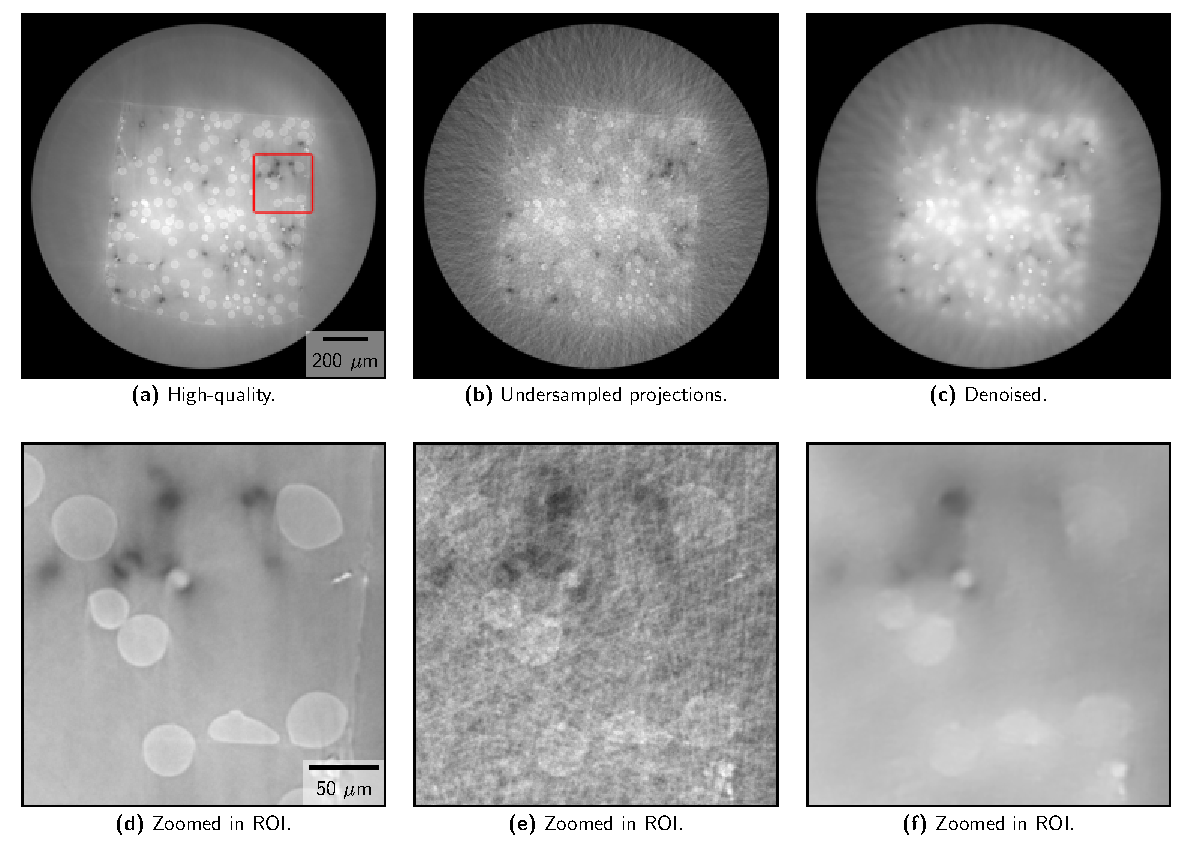
\includegraphics[width=.9\textwidth]{figures/uncroppeddenoising.pdf}
  \caption[Non-cropped image denoising]{Denoising of non-cropped dataset tomo\_00058. Images d), e), and f) are zoomed in \acrshort{roi}s of images a), b), and c) respectively. The \acrshort{roi} is marked in a). }
  \label{fig:uncroppeddenoising}
\end{figure}

\begin{figure}[htbp]
  \centering
  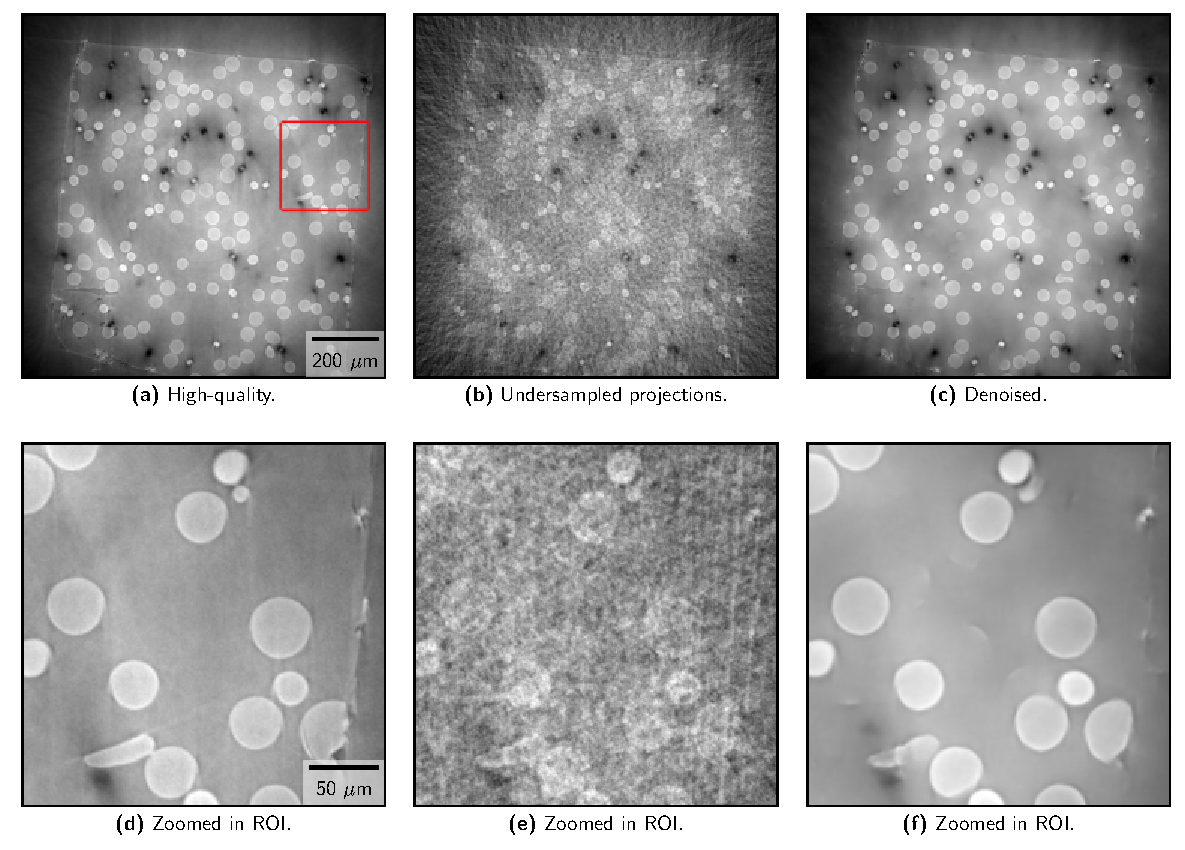
\includegraphics[width=.9\textwidth]{figures/croppeddenoising.pdf}
  \caption[Cropped image denoising]{Denoising of cropped dataset tomo\_00058. Images d), e), and f) are zoomed in \acrshort{roi}s of images a), b), and c) respectively. The \acrshort{roi} is marked in a). }
  \label{fig:croppeddenoising}
\end{figure}

\begin{figure}[htbp]
  \centering
  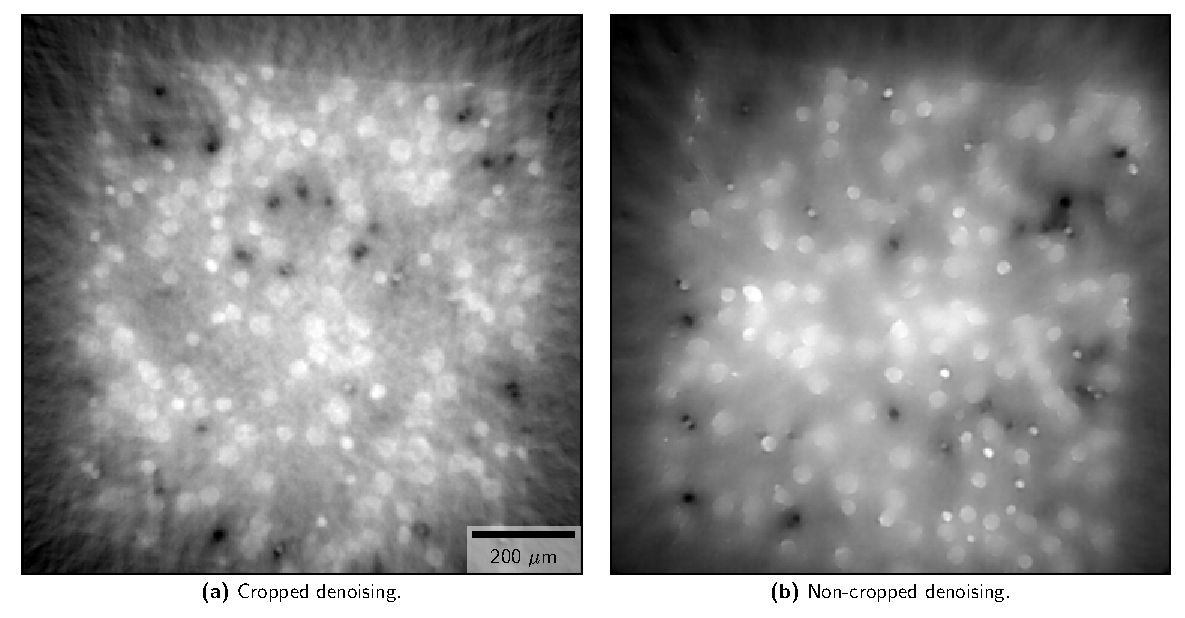
\includegraphics[width=.9\textwidth]{figures/croppednoncroppedearly.pdf}
  \caption[Non-cropped image denoising compared to non-converged cropped image denoising]{Non-cropped image denoising compared to non-converged cropped image denoising. The cropped denoising is after merely $500$ iterations of the same denoising as in \cref{fig:croppeddenoising}. The non-cropped denoising has been cropped after denoising for easier comparison. The two images are of different slices of the same dataset. }
  \label{fig:croppednoncroppedearly}
\end{figure}

\section{Hyperparameter and Loss Function Changes}
\todo[inline]{Show difference in tomo\_00058 denoising for different loss functions / weights (and hyperparameters?)}

\todo[inline]{Line plot of gt, ns, MSE denoising, log-cosh denoising. Multiple lines around the images?}

\todo[inline]{SSIM and MSE evolution of arbitrary slice. }

\section{Different Amounts of Noise}
To explore how much noise the denoising method is able to remove, the tomo\_00058 dataset was recreated with four different levels of missing wedge noise. By using subsampling factors of $8$, $16$, $32$, and $48$ (where the resulting number of projections can be seen in \cref{tab:projectionsubsampling}), four datasets with different levels of noise were simulated. They can be seen alongside the \acrshort{hq} reconstruction in \cref{fig:tomo00058missingwedgecomparison}. 

Once again the TomoGAN network was used with a loss function containing \acrshort{mse}, log-cosh, VGG, and adversarial components, a depth of 1 was used, and the network was trained for 100000 iterations with a mini batch size of 16. The resulting denoised images can be seen in \cref{fig:tomo00058missingwedgecomparisondenoised}. 

It is evident that a subsampling factor of 48, corresponding to merely 31 projections, leads to too much noise to recover any usable denoised image. This is further confirmed by looking at plots of the pixel values along two different lines on the denoised images and comparing them with the noisy and the \acrshort{hq} image, as can be seen in \cref{fig:differentnoiselineplot1,fig:differentnoiselineplot2}. For the other three datasets the denoising seems to result in images sufficiently similar to the \acrshort{hq} image, especially for subsampling factors $8$ and $16$. 

\cref{tab:missingwedgessim} contains \acrshort{ssim} and \acrshort{mse} values for the noisy and denoised images shown in \cref{fig:tomo00058missingwedgecomparison,fig:tomo00058missingwedgecomparisondenoised}. We see here that for subsampling factors $8$, $16$, and $32$, the \acrshort{mse} is improved by denoising, however for subsampling factor $48$ it is drastically worsened. All denoisings achieve, to varying degrees, \acrshort{ssim} improvements. The fact that the poor denoising of the subsampling factor of $48$ achieves an improvement in \acrshort{ssim} from $0.193$ to $0.657$ indicates that \acrshort{ssim} is not a perfect image comparison metric. 

It is worth noting that a subsampling factor of $32$ corresponds to $46$ projections, which is similar to the $64$ projections used in the noisiest simulated dataset in the original article by Liu et al. \cite{liu2020tomogan}. The achieved \acrshort{ssim} score on a real dataset of $0.789$ in this thesis is similar to their results on a simulated phantom. 

\todo[inline]{Plot showing improvement in SSIM for different levels of noise. }



\begin{figure}
  \begin{subfigure}[t]{\textwidth}
    \centering
    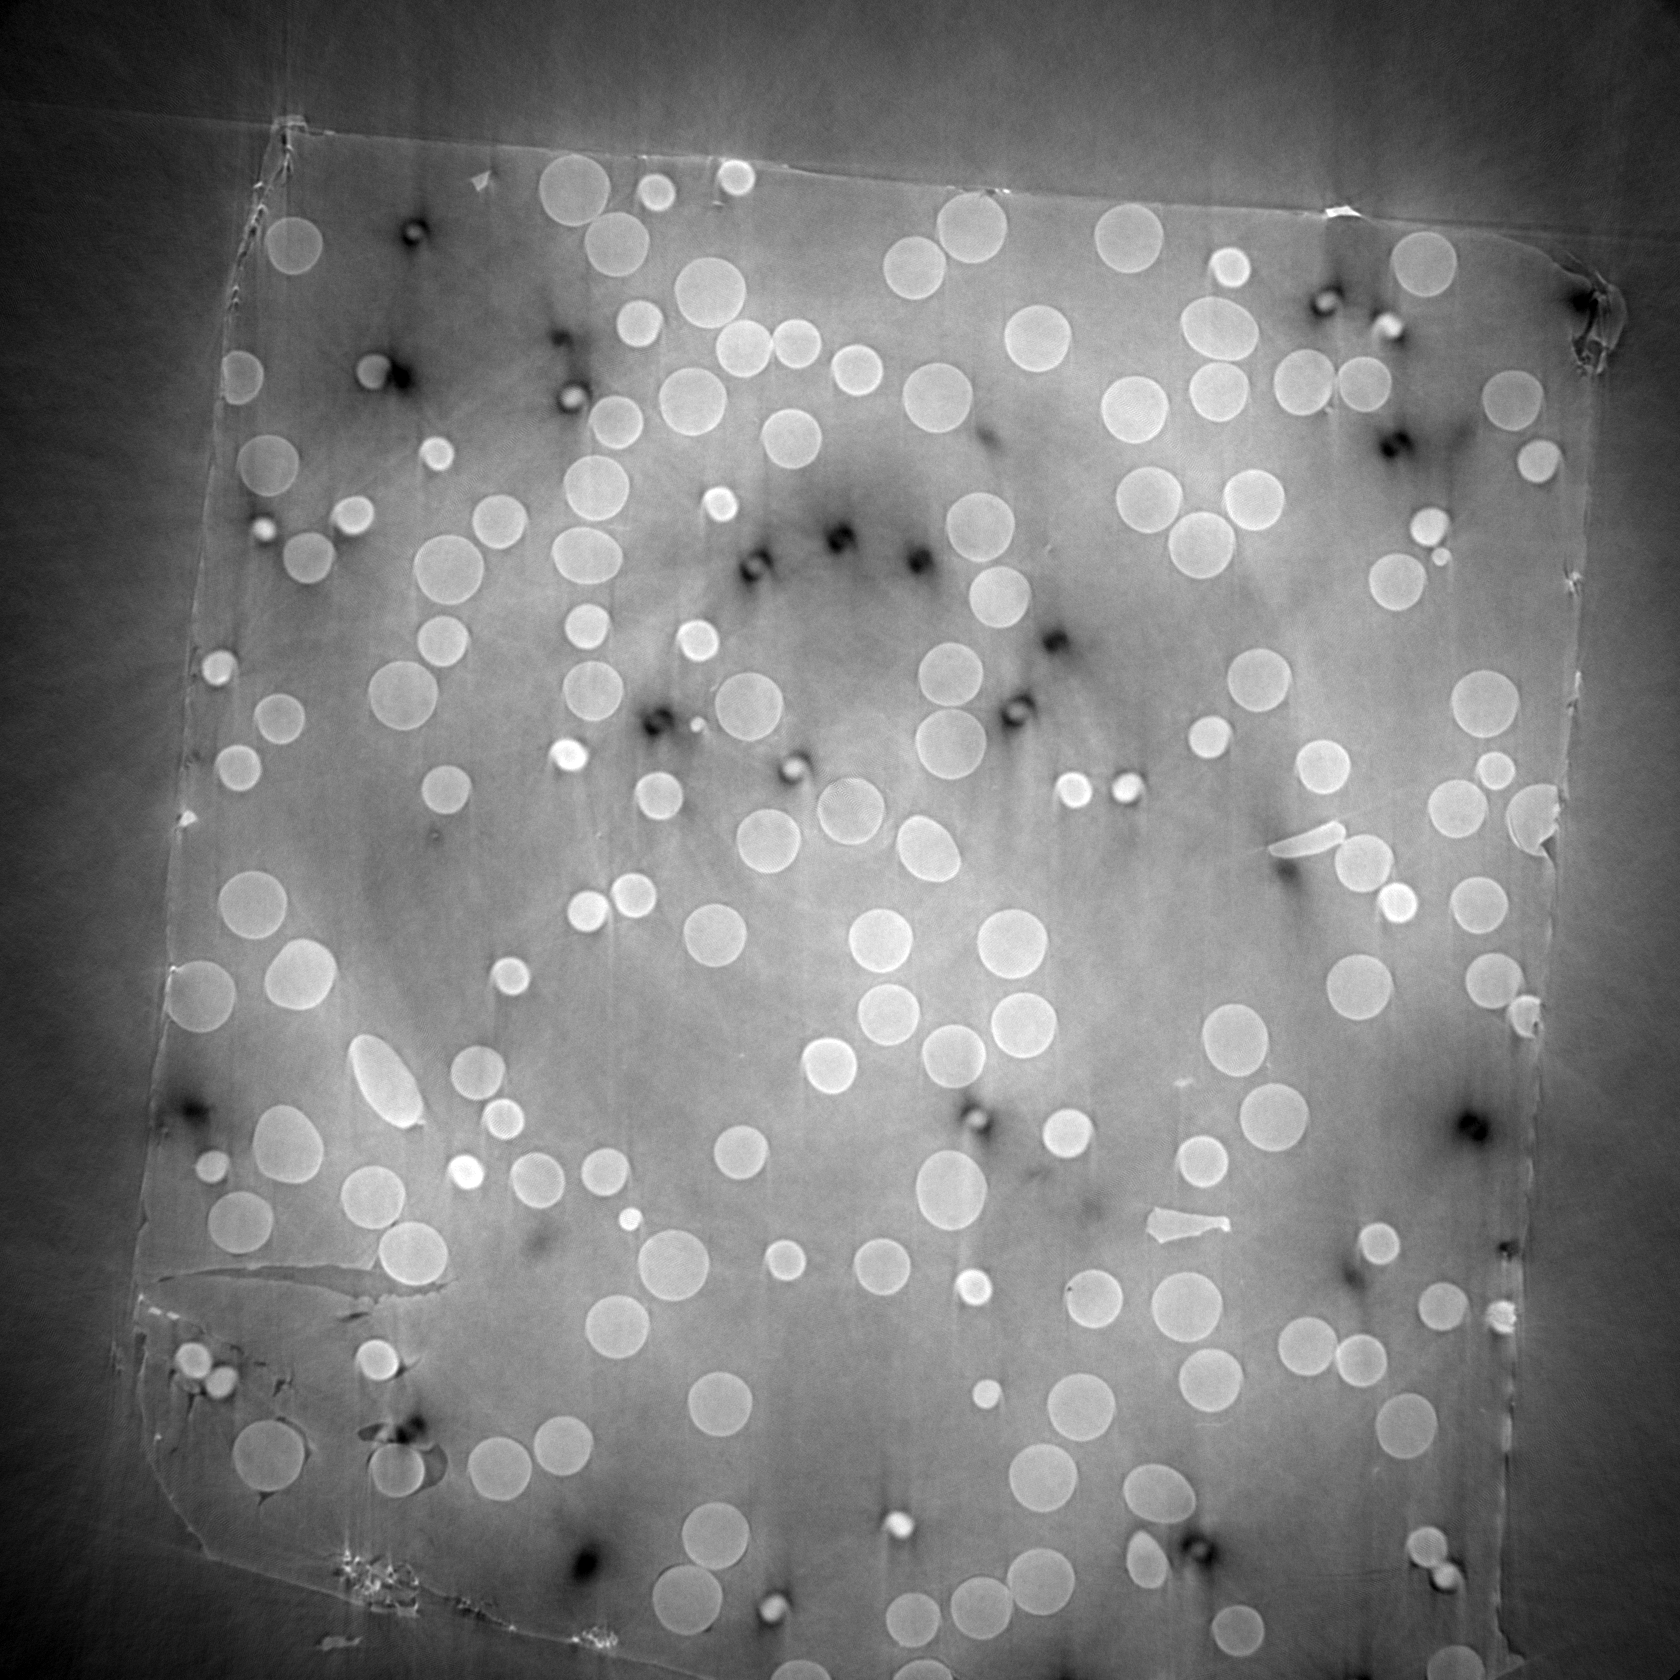
\includegraphics[width=.45\textwidth]{figures/gt32.png}
    \caption{\acrlong{hq}. }
  \end{subfigure}

  \medskip

  \begin{subfigure}[t]{.45\textwidth}
    \centering
    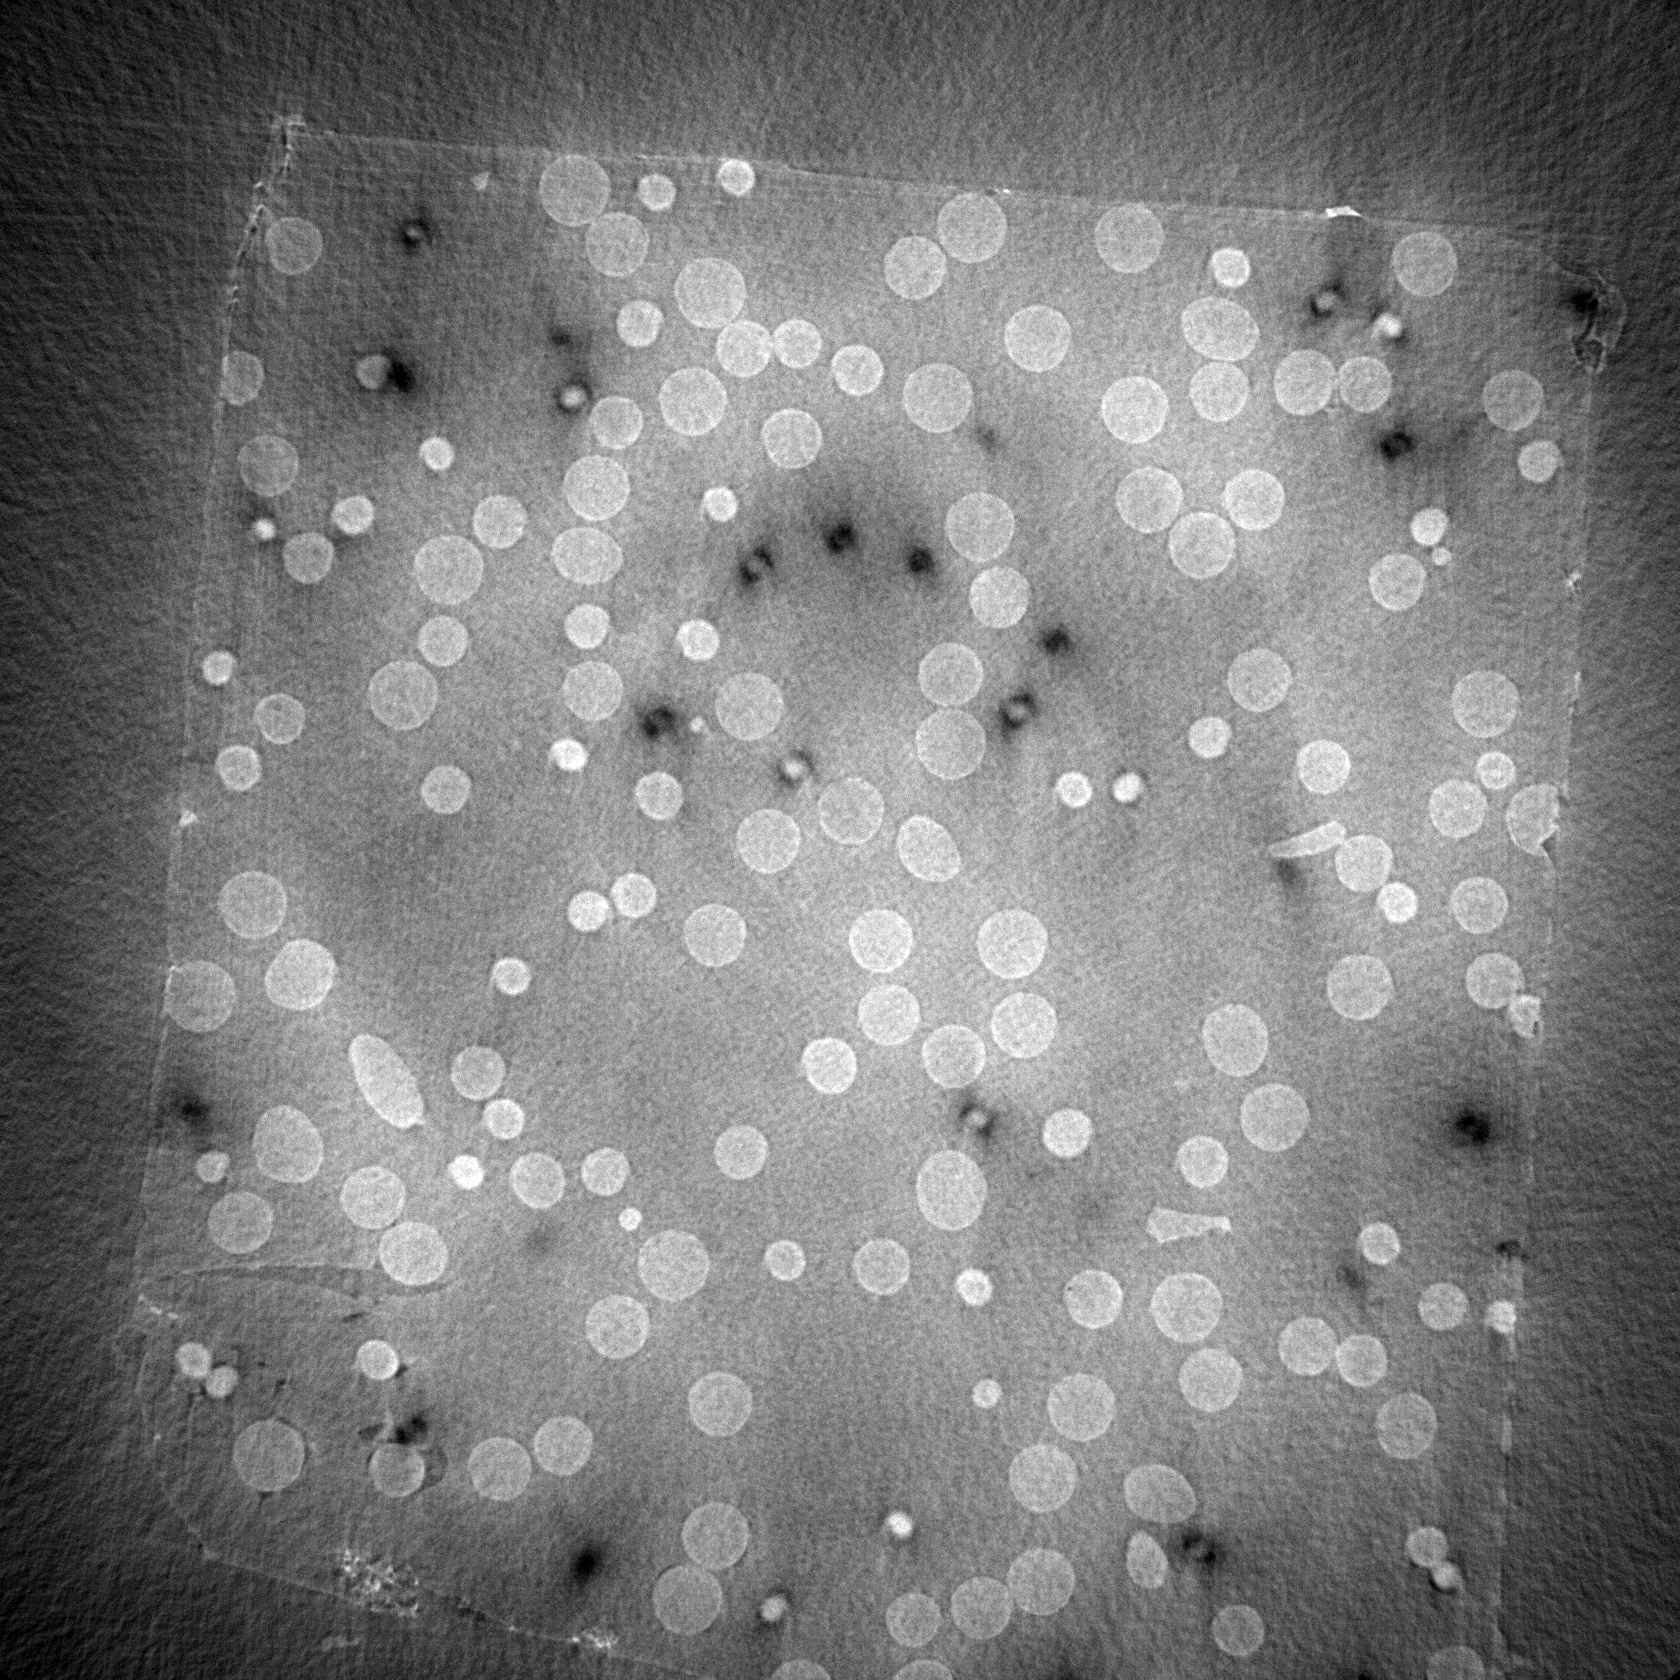
\includegraphics[width=\linewidth]{figures/ns8.png}
    \caption{Subsampling factor 8. }
  \end{subfigure}
  \hfill
  \begin{subfigure}[t]{.45\textwidth}
    \centering
    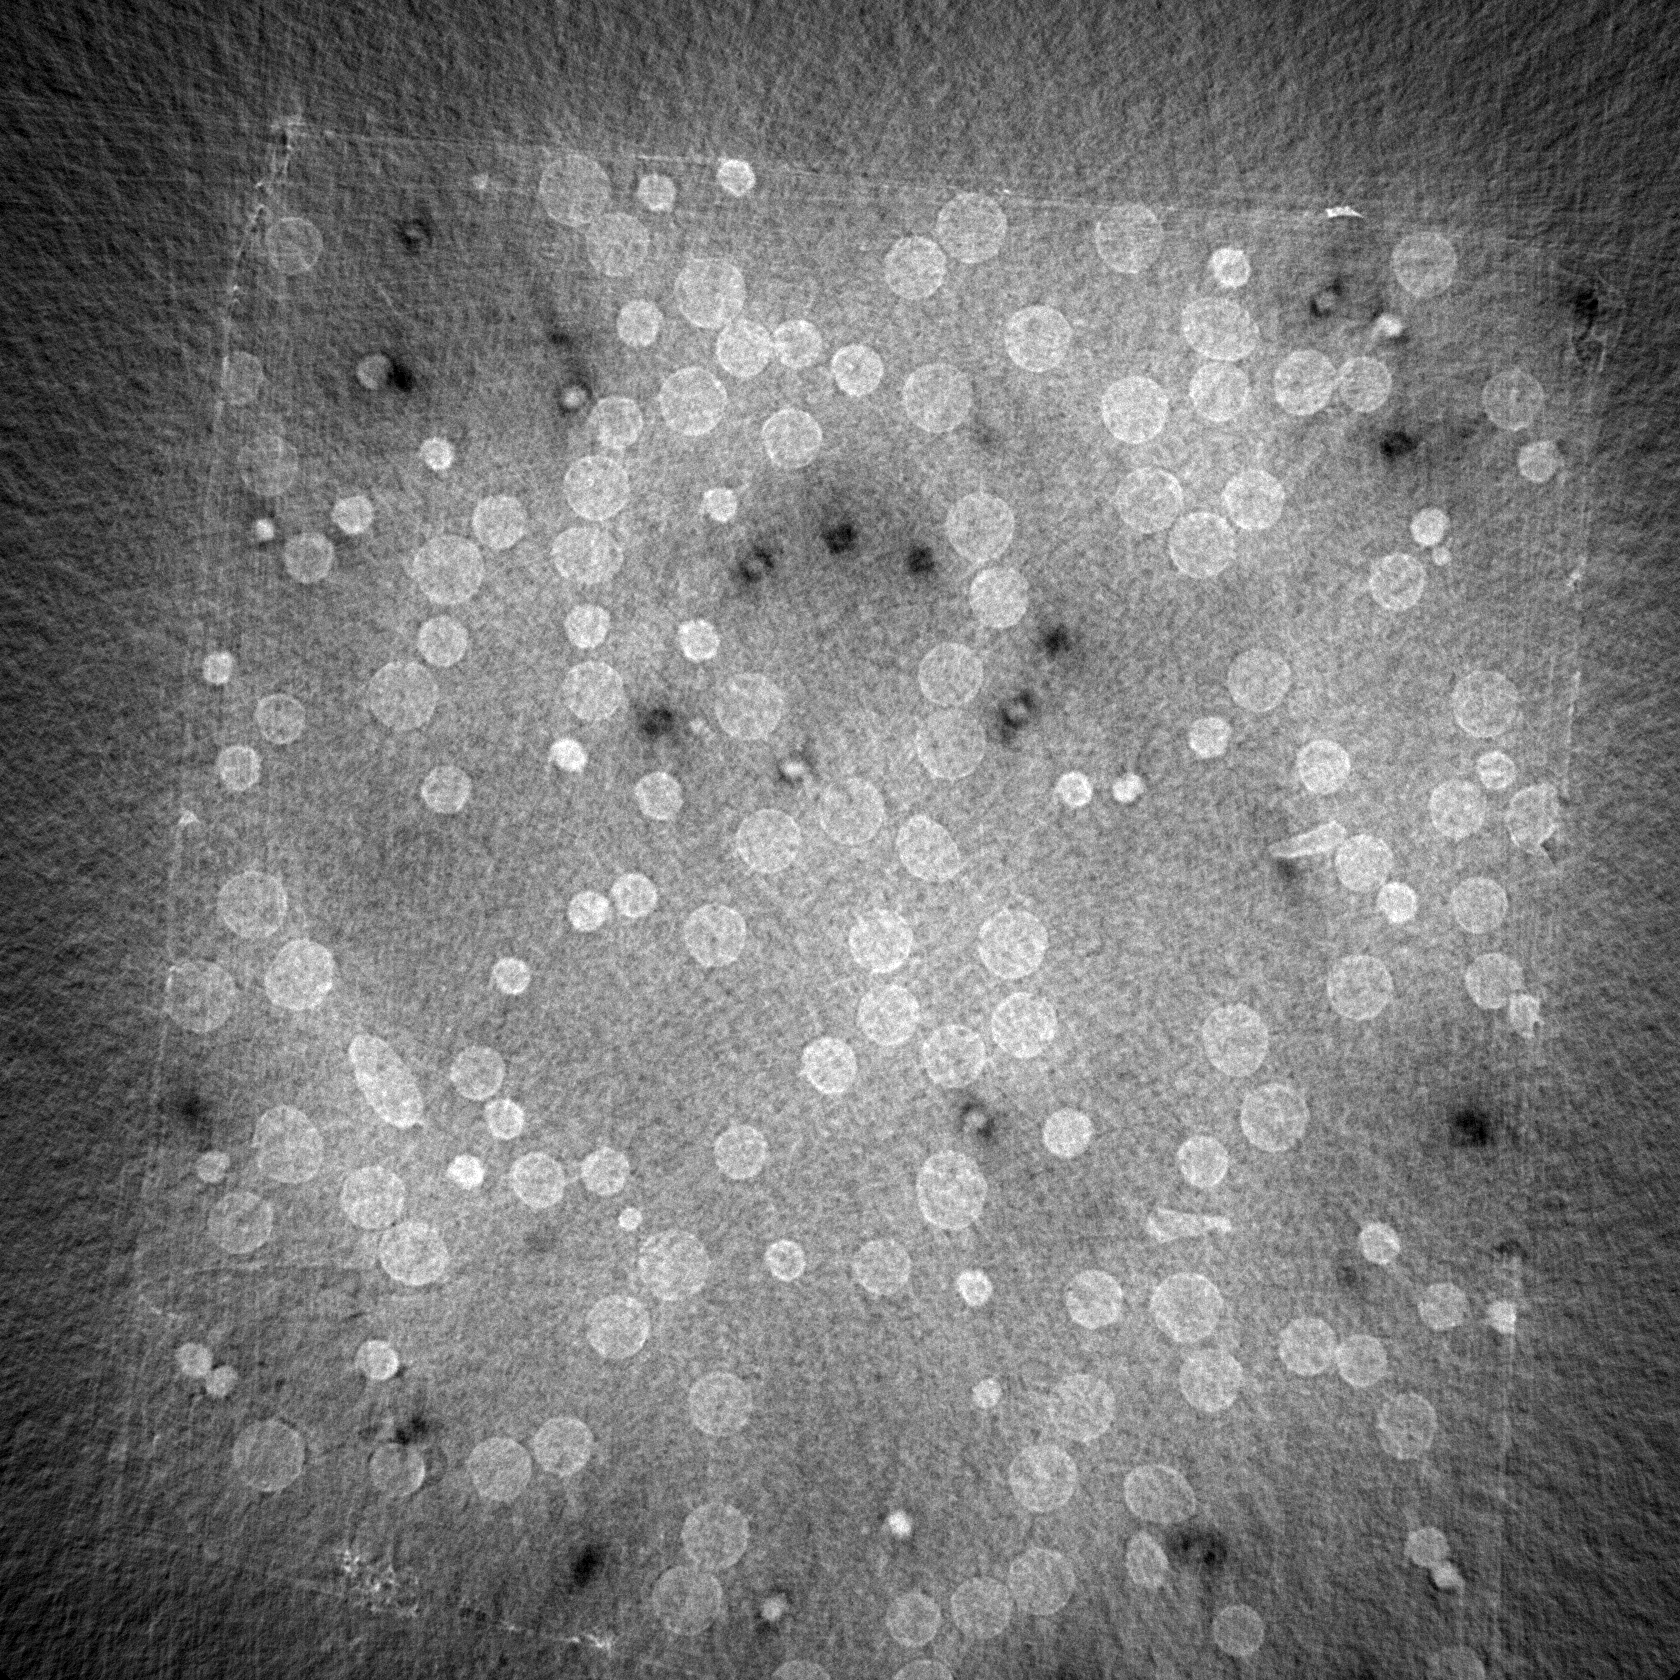
\includegraphics[width=\linewidth]{figures/ns16.png}
    \caption{Subsampling factor 16. }
  \end{subfigure}

  \medskip

  \begin{subfigure}[t]{.45\textwidth}
    \centering
    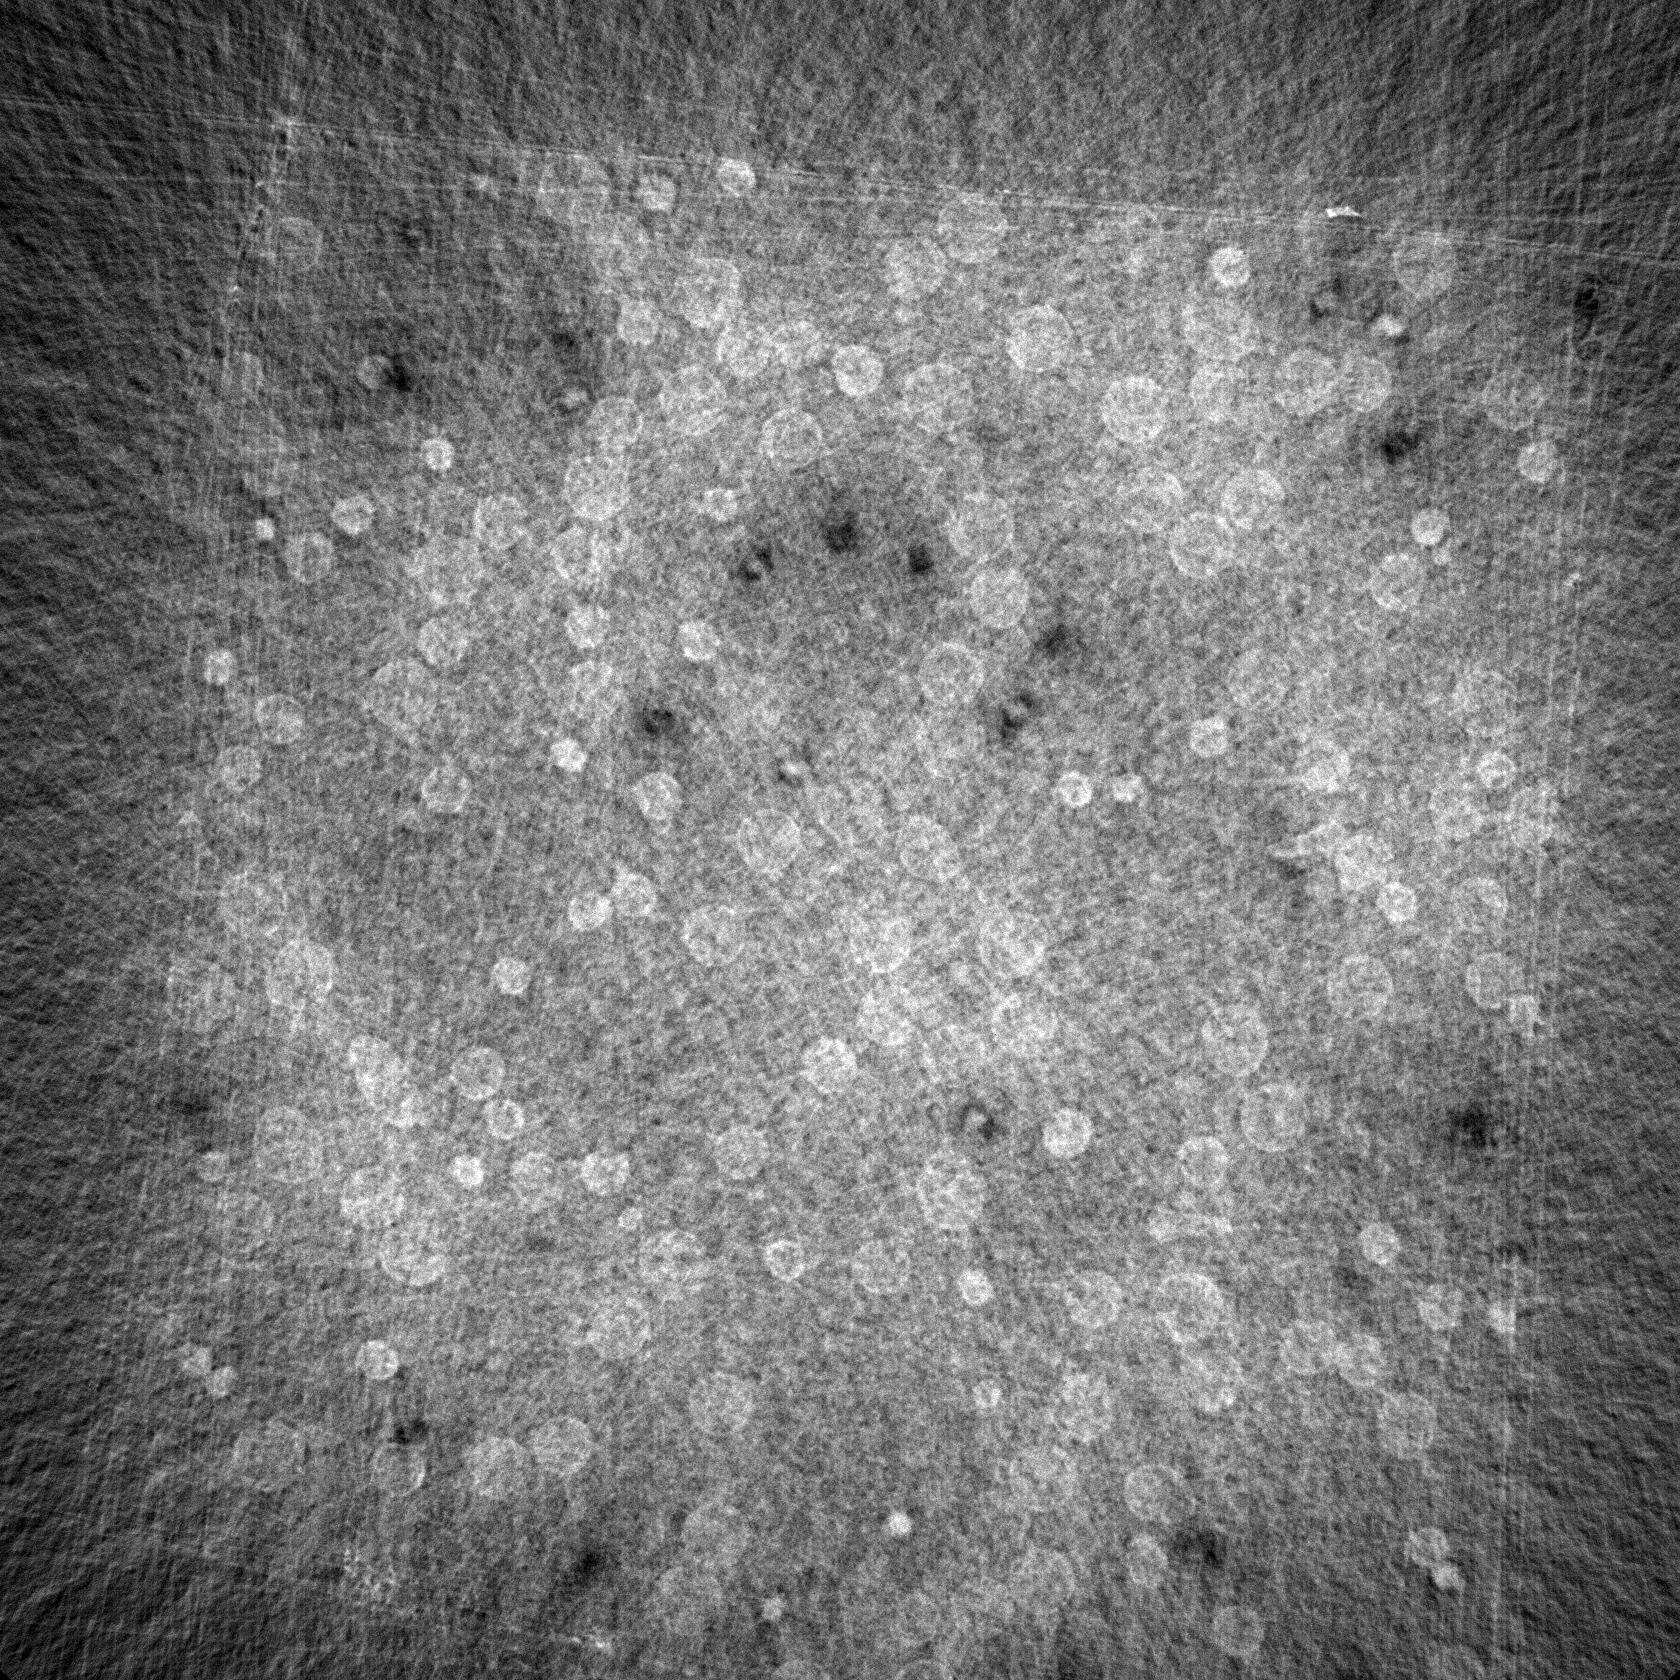
\includegraphics[width=\linewidth]{figures/ns32.png}
    \caption{Subsampling factor 32. }
  \end{subfigure}
  \hfill
  \begin{subfigure}[t]{.45\textwidth}
    \centering
    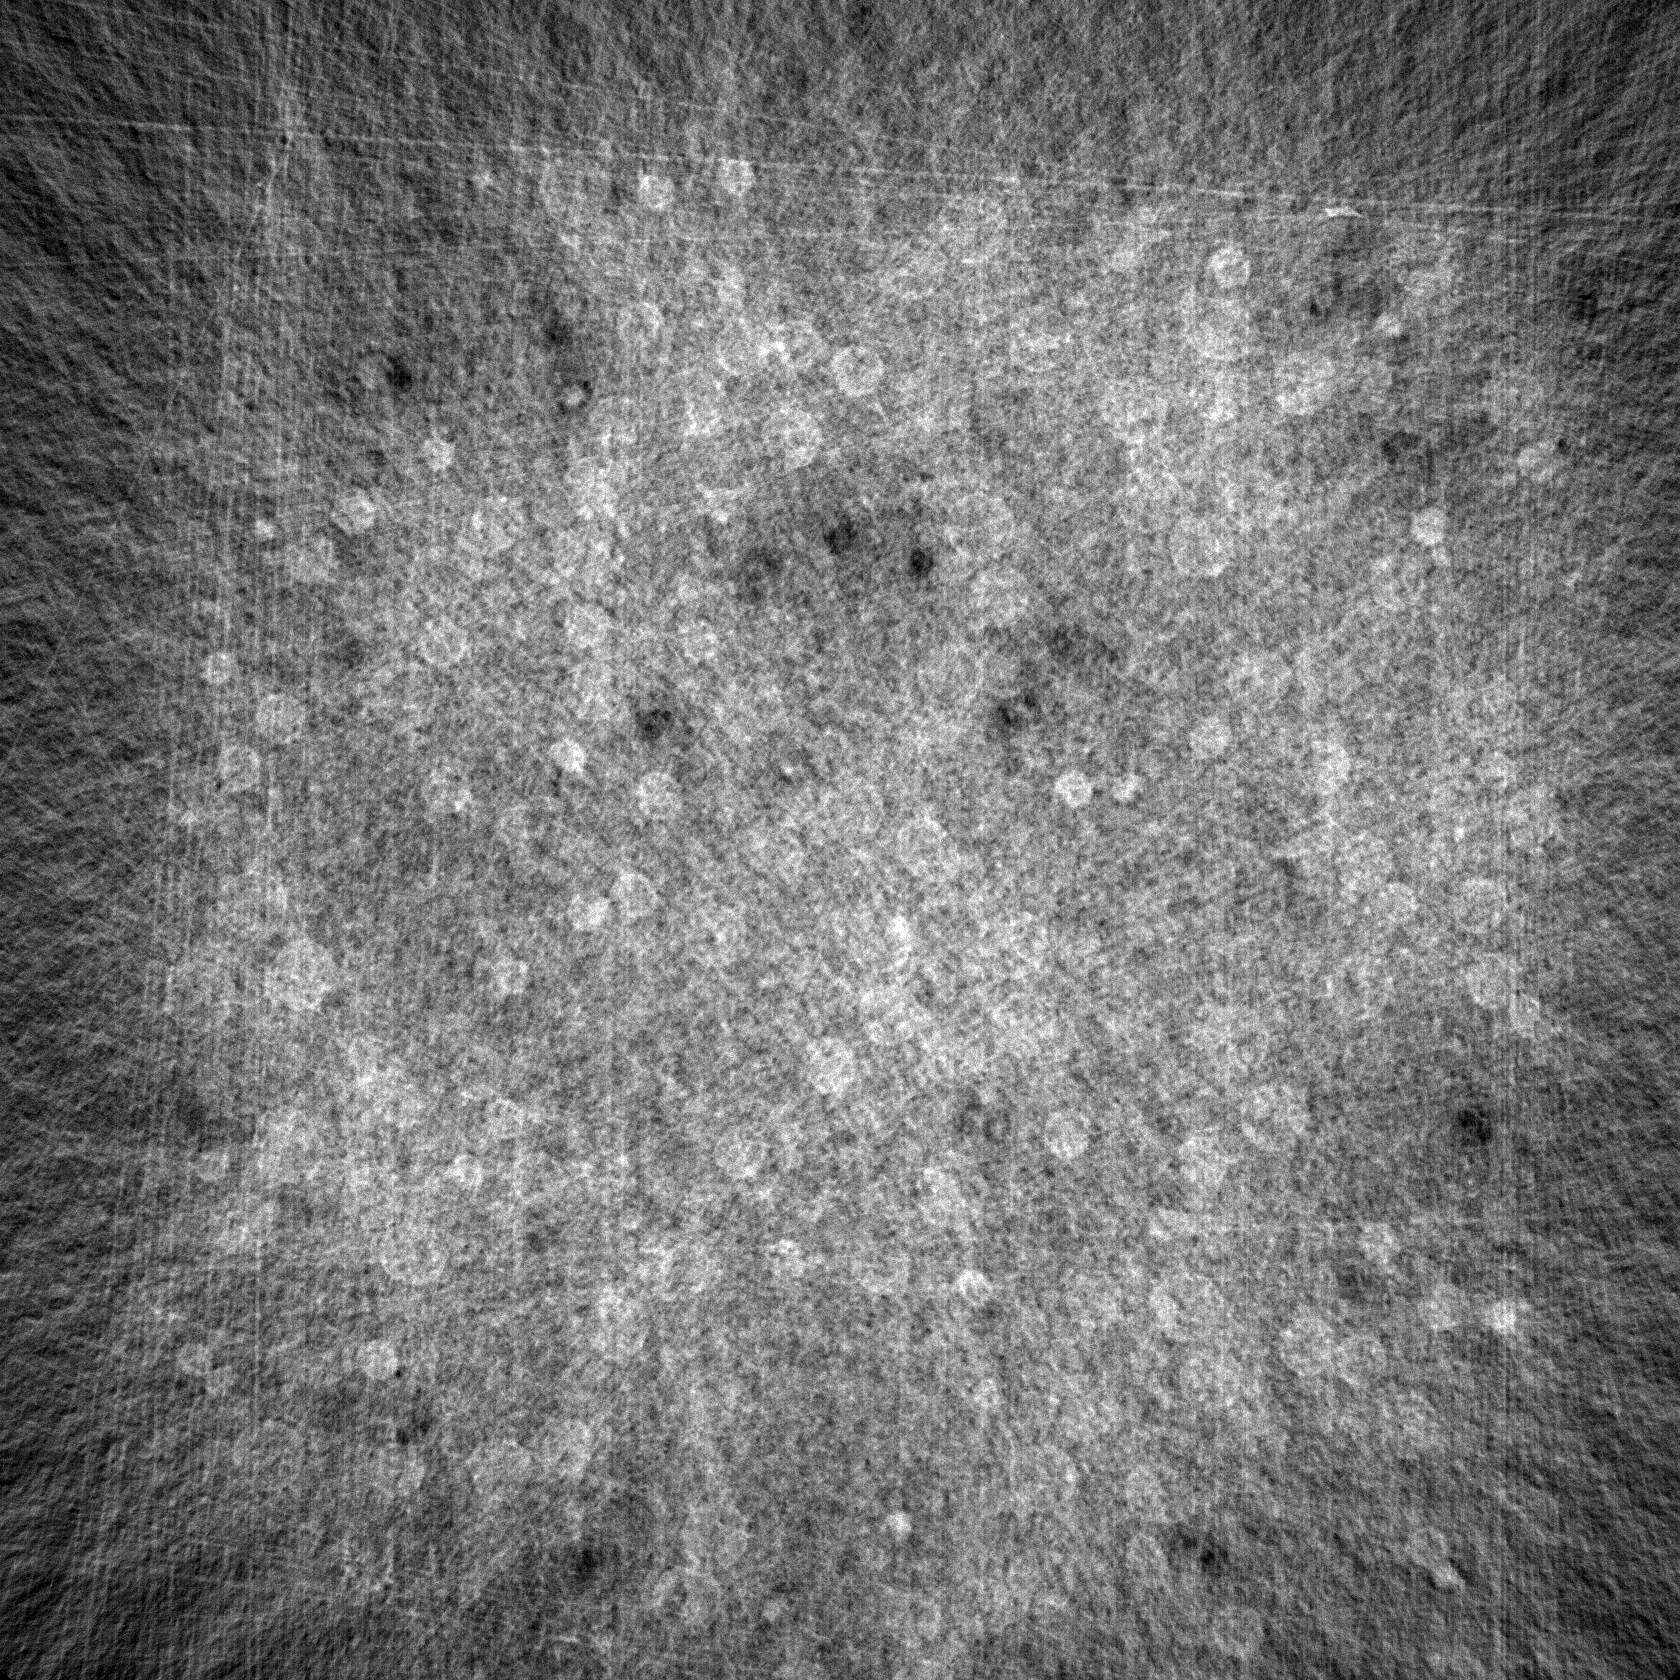
\includegraphics[width=\linewidth]{figures/ns48.png}
    \caption{Subsampling factor 48. }
  \end{subfigure}
  \caption[Four different levels of missing wedge noise]{Comparison of different levels of missing wedge noise on the tomo\_00058 dataset. The four noisy images have been reconstructed with \acrshort{fbp} with different levels of subsampling of the projections, leading to noise. The number of projections corresponding to a given subsampling factor can be seen in \cref{tab:projectionsubsampling}. }
  \label{fig:tomo00058missingwedgecomparison}
\end{figure}


\begin{figure}
  \begin{subfigure}[t]{.45\textwidth}
    \centering
    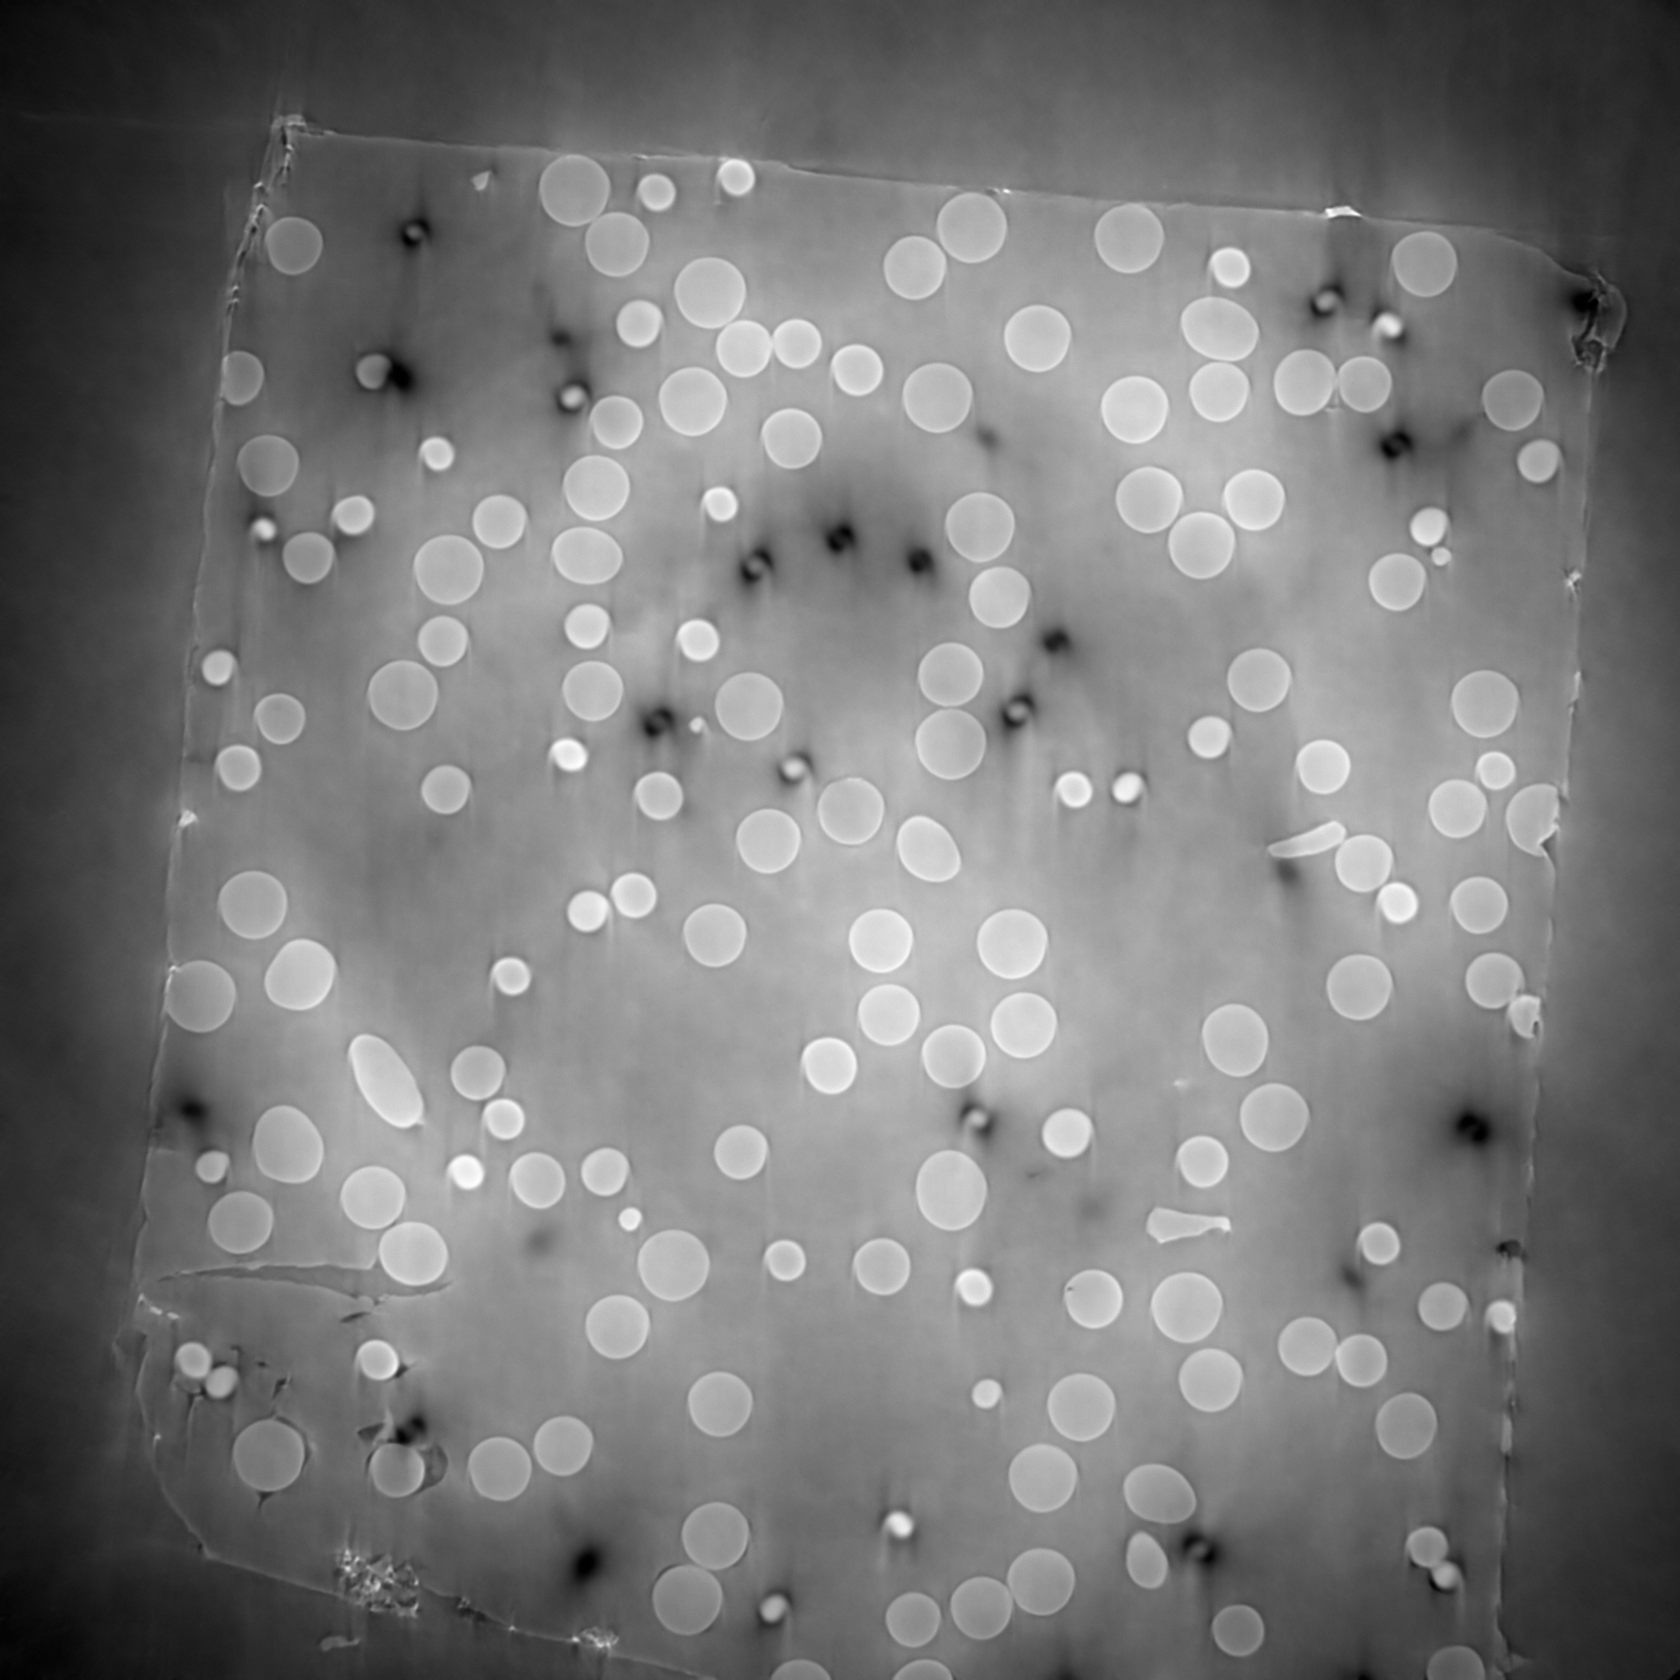
\includegraphics[width=\linewidth]{figures/ns8it100000itd4mse035logcosh3.png}
    \caption{Subsampling factor 8. }
  \end{subfigure}
  \hfill
  \begin{subfigure}[t]{.45\textwidth}
    \centering
    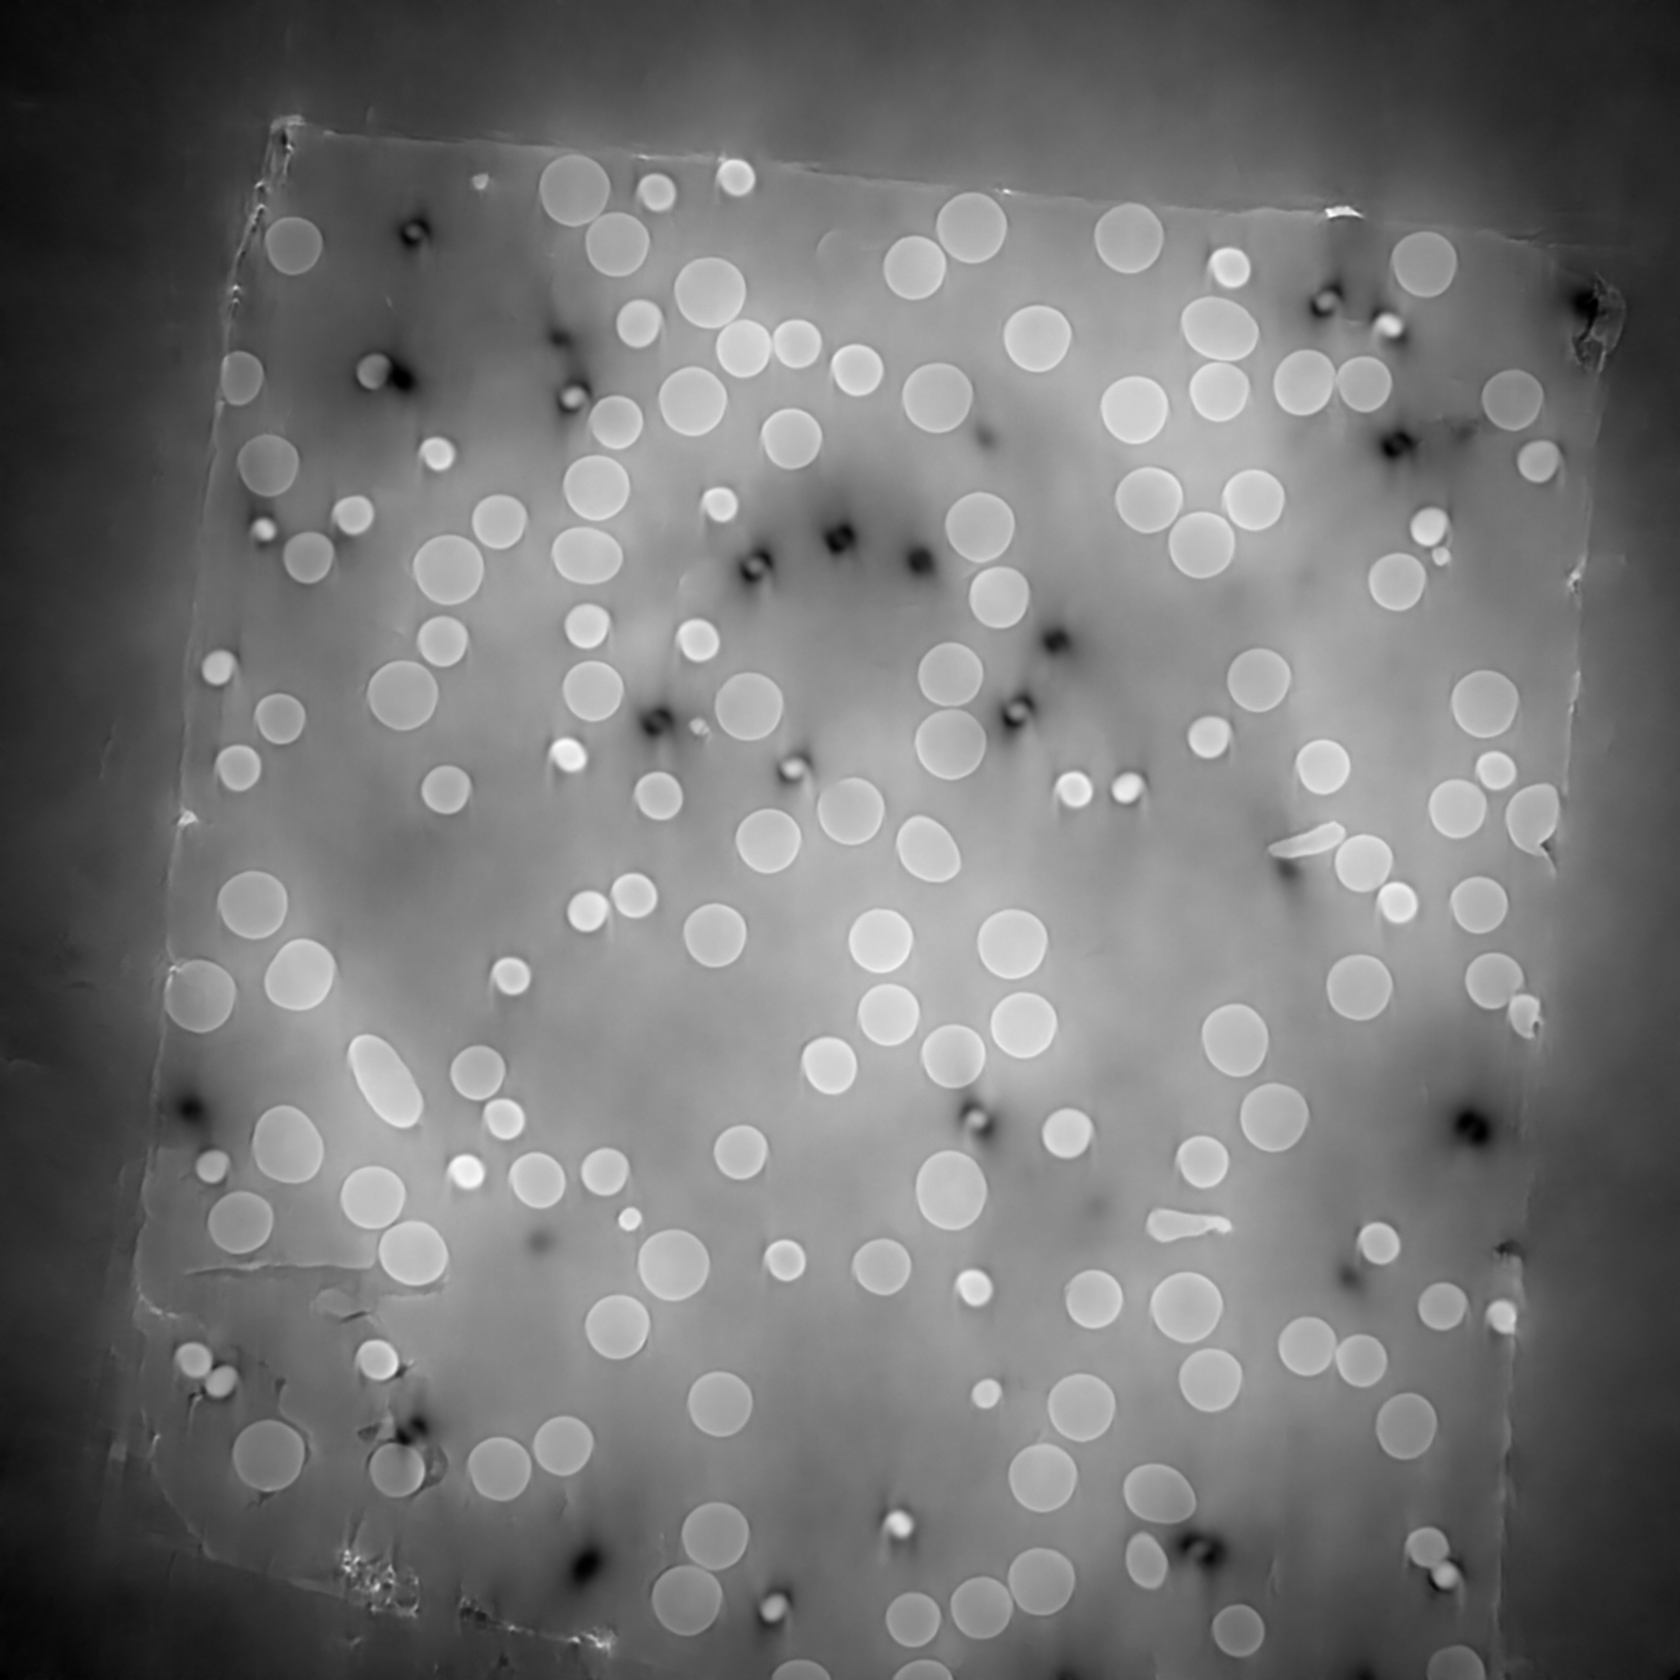
\includegraphics[width=\linewidth]{figures/ns16it100000itd4mse035logcosh3.png}
    \caption{Subsampling factor 16. }
  \end{subfigure}

  \medskip

  \begin{subfigure}[t]{.45\textwidth}
    \centering
    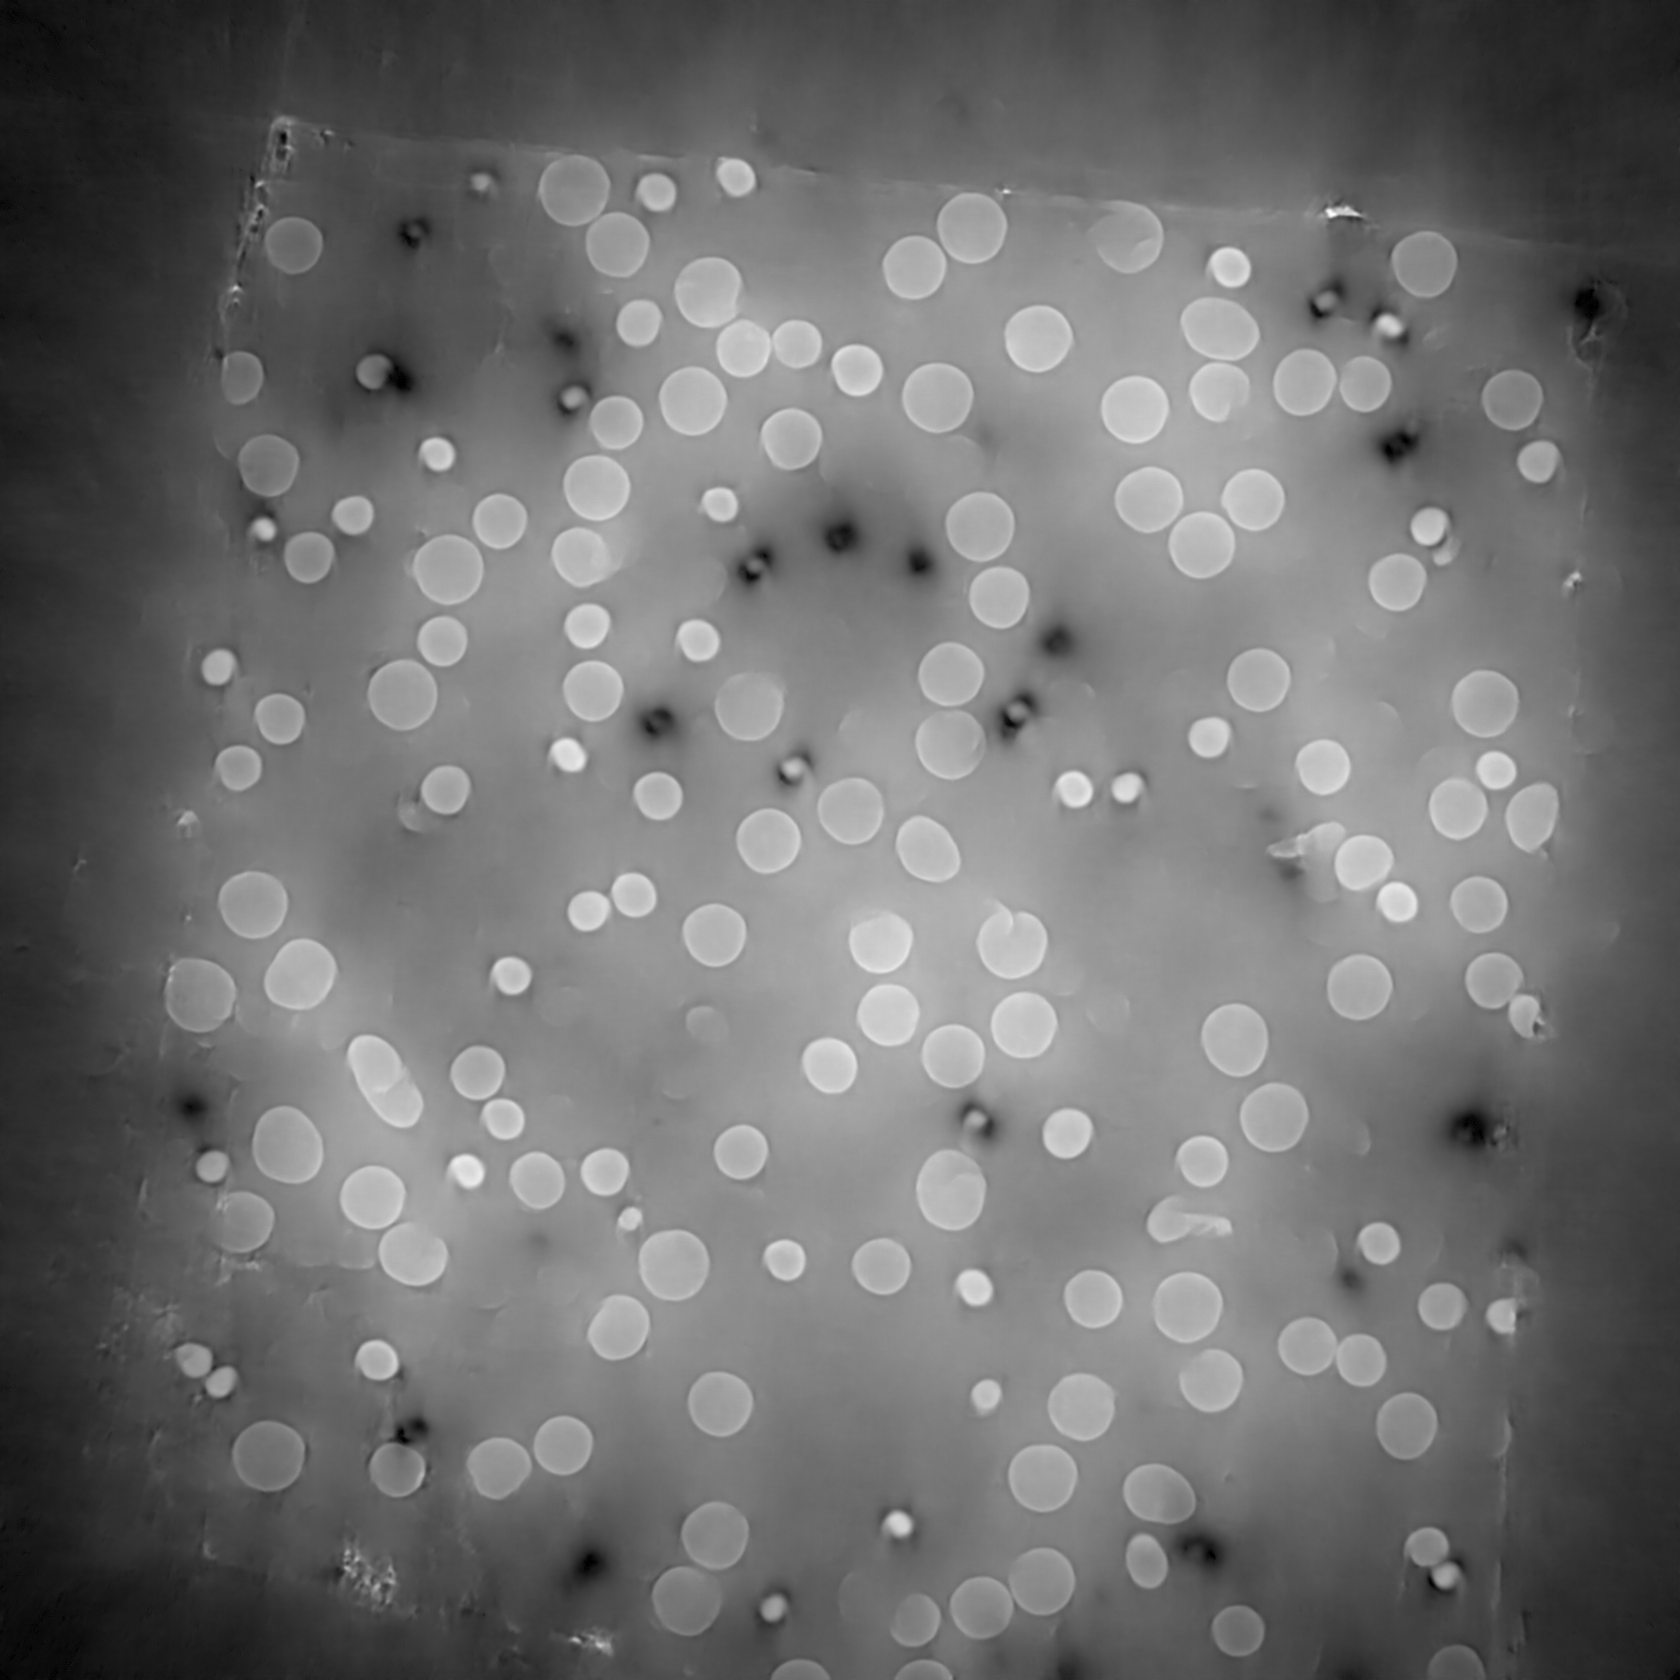
\includegraphics[width=\linewidth]{figures/ns32it100000itd4mse035logcosh3.png}
    \caption{Subsampling factor 32. }
  \end{subfigure}
  \hfill
  \begin{subfigure}[t]{.45\textwidth}
    \centering
    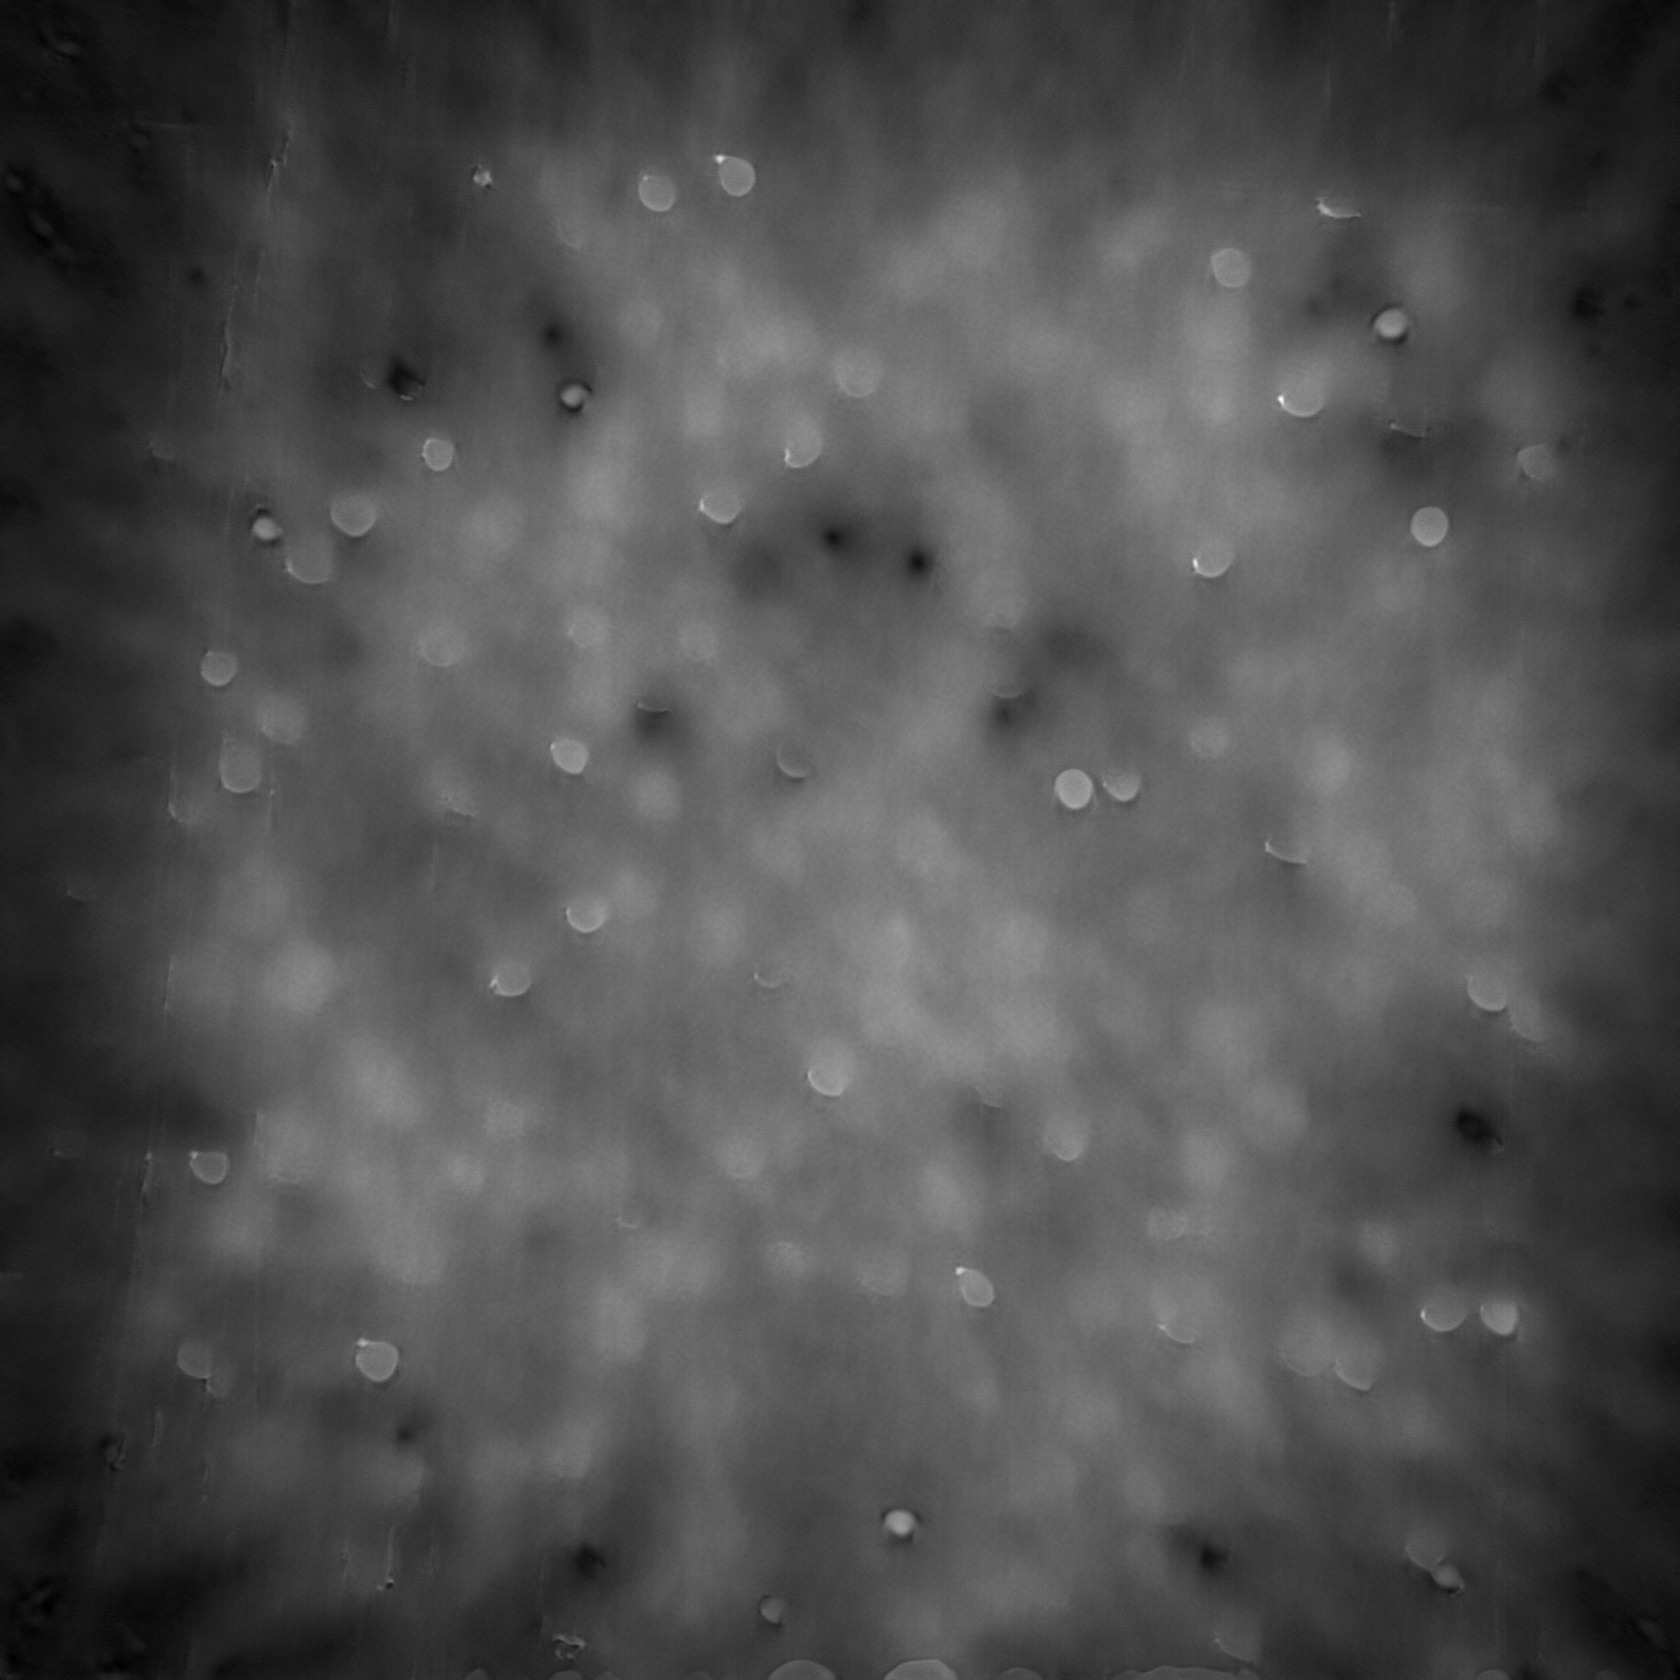
\includegraphics[width=\linewidth]{figures/ns48it100000itd4mse035logcosh3.png}
    \caption{Subsampling factor 48. }
  \end{subfigure}
  \caption[Denoising of four different levels of missing wedge noise]{Comparison of denoising of different levels of missing wedge noise on the tomo\_00058 dataset, where the corresponding noisy images can be seen in \cref{fig:tomo00058missingwedgecomparison}. The denoising was done with TomoGAN using a loss function containing \acrshort{mse}, log-cosh, VGG, and adversarial loss components, a depth of 1, and the network was trained for $100 000$ iterations. }
  \label{fig:tomo00058missingwedgecomparisondenoised}
\end{figure}


\begin{table}[htbp]
  \centering
  \caption[SSIM for different levels of simulated missing wedge noise and corresponding values after denoising]{Overview of \acrshort{ssim} for different levels of simulated missing wedge noise on the tomo\_00058 dataset. The missing wedge noise was simulated by subsampling the number of projections by a factor as given in the subsampling factor column, which results in a number of projections as given in \cref{tab:projectionsubsampling}. All denoising was done with TomoGAN using a loss function containing \acrshort{mse}, log-cosh, VGG, and adversarial loss components, a depth of 1, and the network was trained for $100 000$ iterations. }
  \label{tab:missingwedgessim}
  \begin{tabular}{lllll}
  \hline
  \multirow{2}{*}{Subsampling Factor} & \multicolumn{2}{c}{\acrshort{ssim}} & \multicolumn{2}{c}{\acrshort{mse}}  \\
  {} & Noisy & Denoised & Noisy & Denoised \\
  \hhline{=====}
  %\hline 
  $1$  & $1.0$ & $-$ & $0.0$ & $-$ \\
  $8$  & $0.492$ & $0.842$ & $148.3$ & $33.3$ \\
  $16$ & $0.335$ & $0.816$ & $348.5$ & $74.9$ \\
  $32$ & $0.233$ & $0.789$ & $704.4$ & $210.8$ \\
  $48$ & $0.193$ & $0.657$ & $976.6$ & $2362.6$ \\
  \hline
  \end{tabular}
\end{table}

\begin{figure}[htbp]
  \centering
  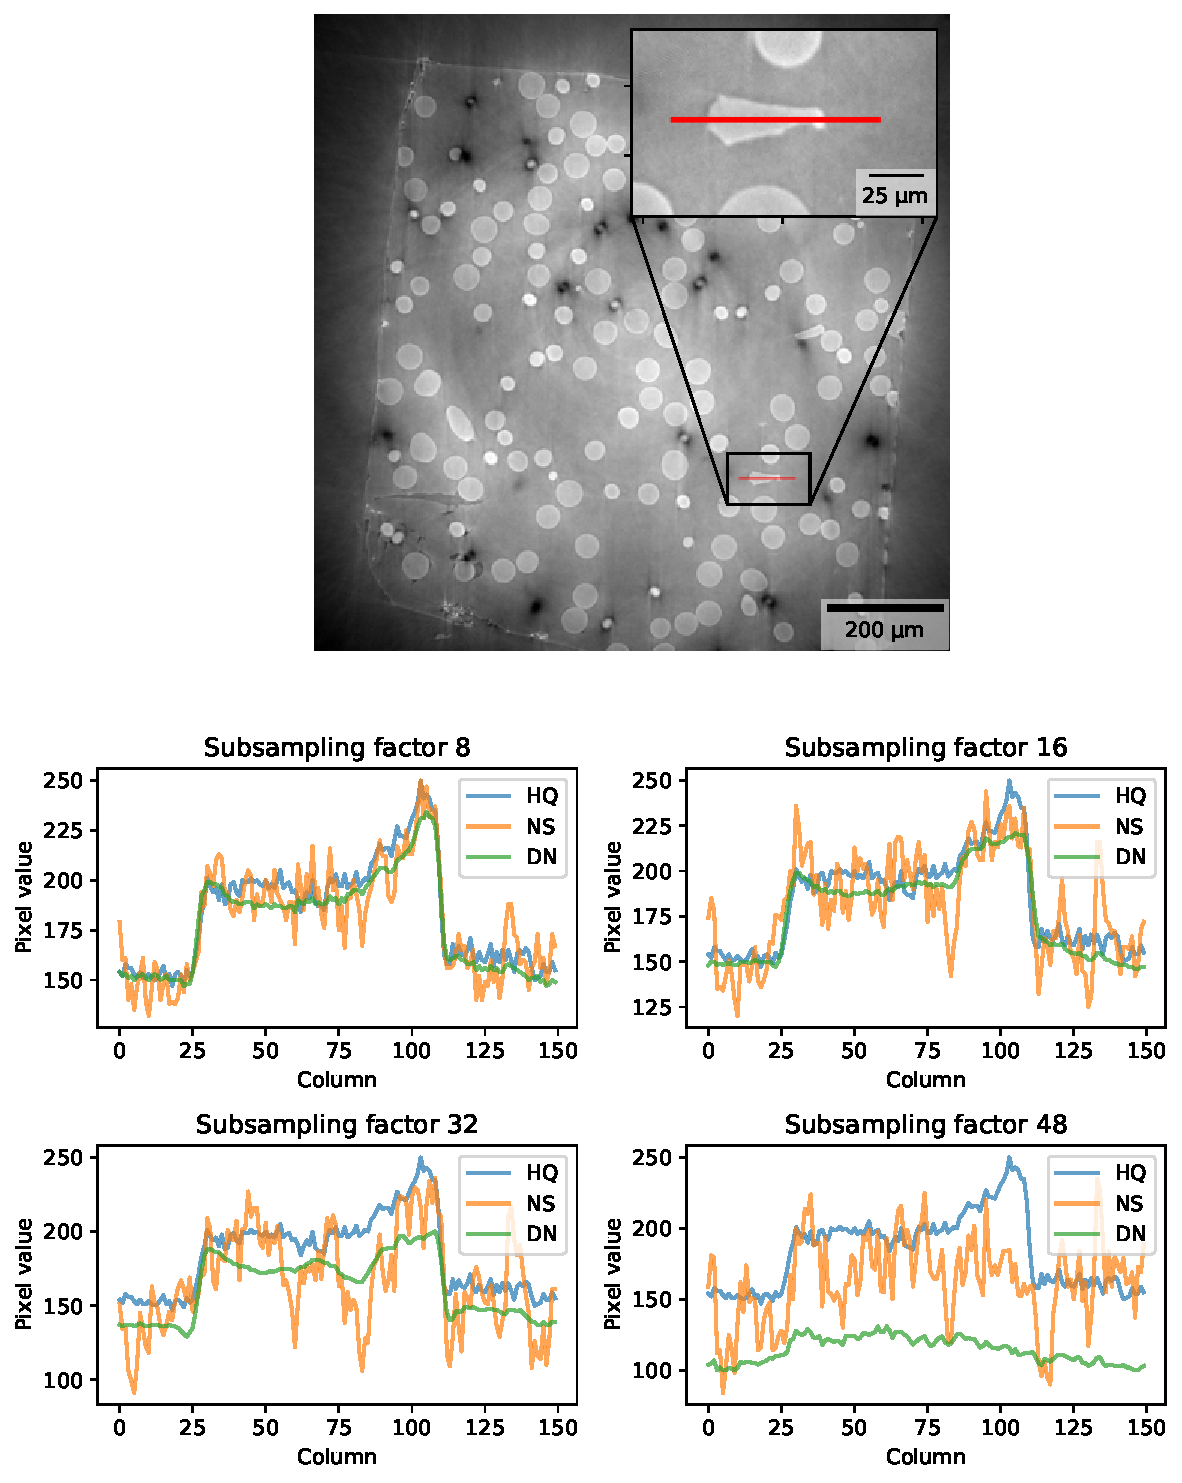
\includegraphics[width=.95\textwidth]{figures/differentnoiselineplot1.pdf}
  \caption[Line plot of denoising of different levels of noise on tomo\_00058]{The plots show pixel values for 150 pixels on a horizontal line on the tomo\_00058 dataset, as shown by the red line on the \acrlong{hq} image above, for denoising of four different levels of missing wedge noise. \acrshort{hq} corresponds to the \acrlong{hq} image, NS to the missing wedge noise image, and \acrshort{dn} to the \acrfull{dn} image. All denoising was done with TomoGAN using a loss function containing \acrshort{mse}, log-cosh, VGG, and adversarial loss components, a depth of 1, and the network was trained for $100 000$ iterations. }
  \label{fig:differentnoiselineplot1}
\end{figure}

\begin{figure}[htbp]
  \centering
  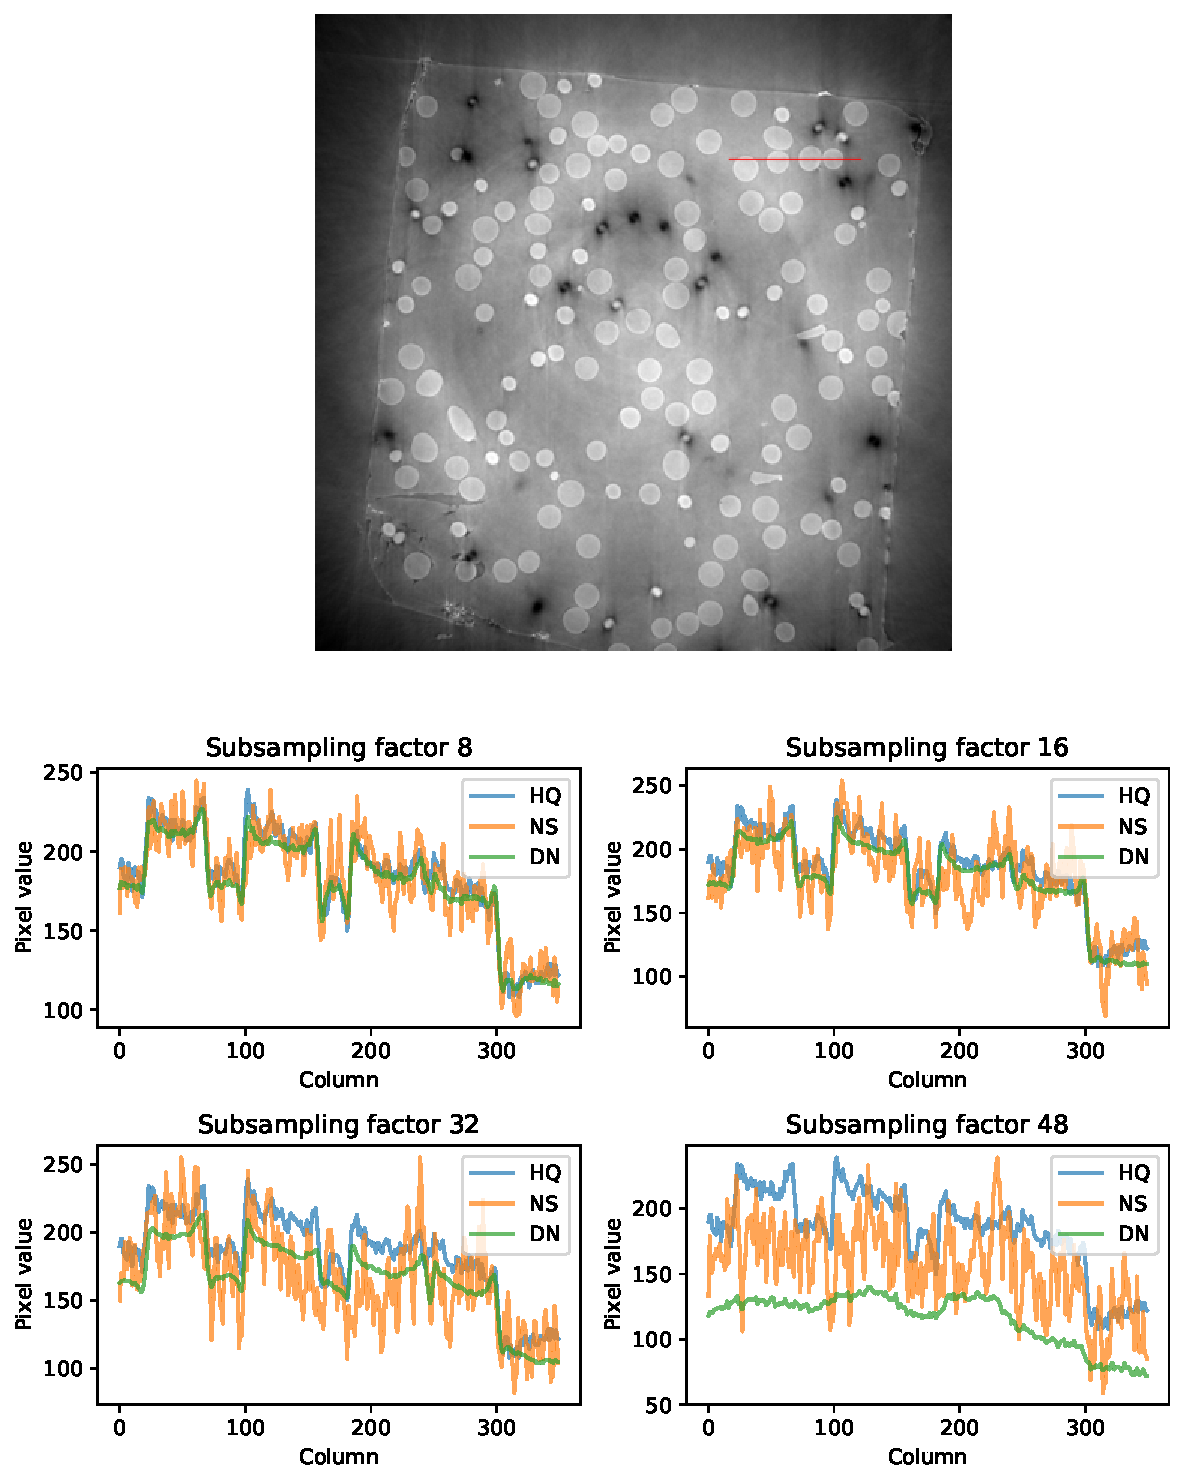
\includegraphics[width=.95\textwidth]{figures/differentnoiselineplot2.pdf}
  \caption[Line plot of denoising of different levels of noise on tomo\_00058]{The plots show pixel values for 400 pixels on a horizontal line on the tomo\_00058 dataset, as shown by the red line on the \acrshort{hq} image above, for denoising of four different levels of missing wedge noise. Figure elements are as in \cref{fig:differentnoiselineplot1}. }
  \label{fig:differentnoiselineplot2}
\end{figure}

\section{Loss Function Evolution}
\todo[inline]{Plot how loss functions evolve through training of tomo\_00058 with good hyperparameters. }

\begin{figure}[htbp]
  \centering
  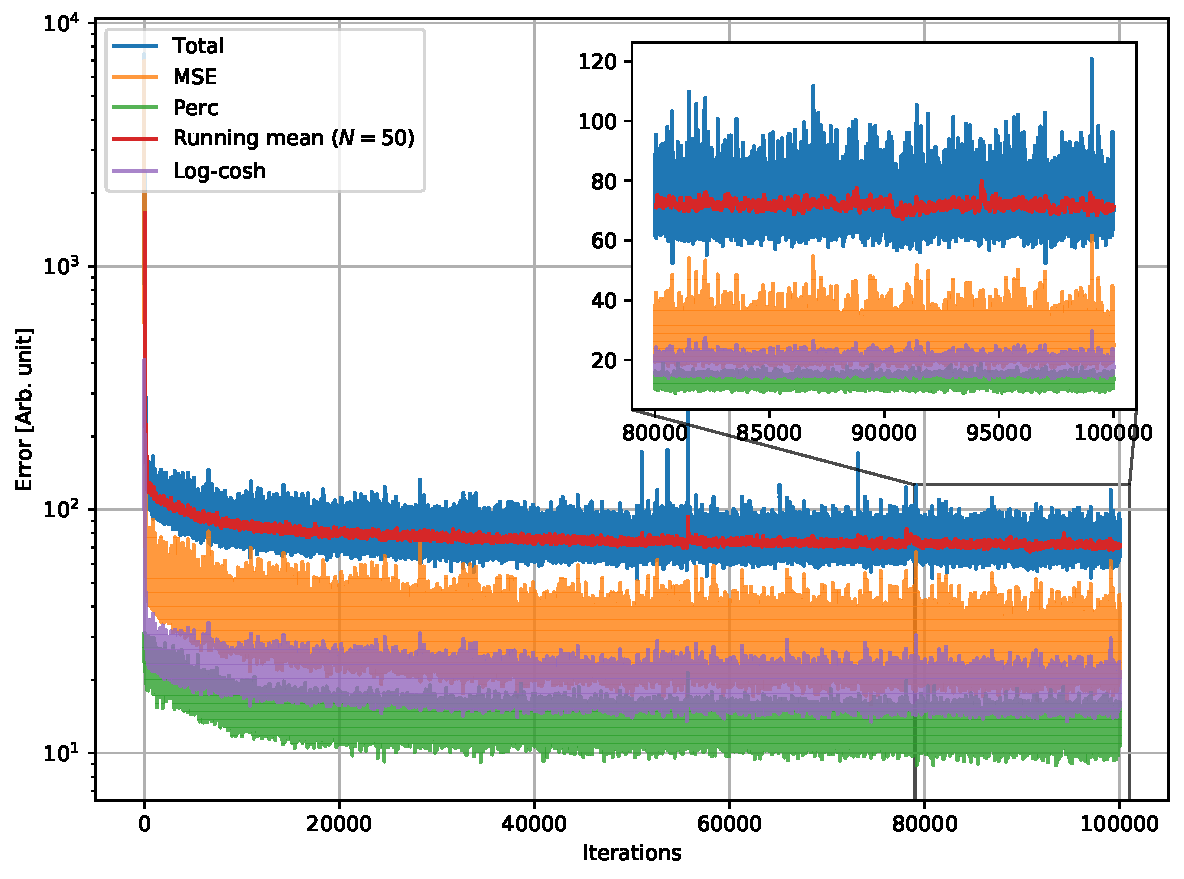
\includegraphics[width=.85\textwidth]{figures/losstomo00058ns32itd4mse035logcosh3depth1.pdf}
  \caption[Loss function evolution]{Loss function evolution. } 
  \label{fig:losstomo00058noadv}
\end{figure}


\section{TomoGAN Compared to PICCS}
\todo[]{Change section name?}
\todo[inline]{Axial, sagittal, coronal plots for different depth parameters. }
\todo[inline]{Maybe make 3D model plot of this dataset. }
\todo[inline]{Line plot comparing GT, FDK?, PICCS, denoised. }
\todo[inline]{Histogram. Looks like peaks roughly align, sharper peaks. Looks like it is performing segmentation? Note: ordinate (y-axis) cropped to 20k. }

\cref{fig:kimrobertcomparison,fig:sideplothq,fig:sideplotfdk,fig:sideplotpiccs,fig:sideplotdepth1,fig:sideplotdepth3,fig:sideplotdepth5,fig:sideplotdepth7,fig:kimrobertline,fig:kimroberthist}. 

\begin{figure}
    \begin{subfigure}[t]{.45\textwidth}
      \centering
      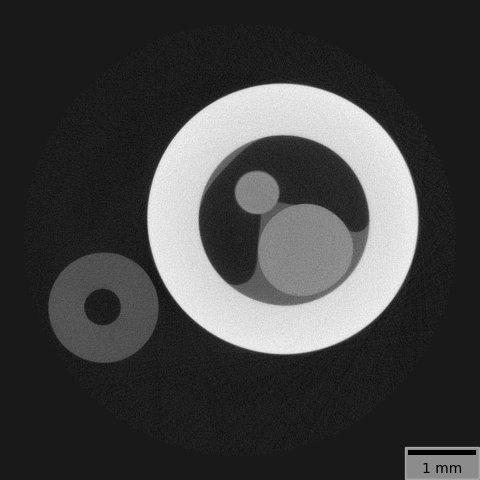
\includegraphics[width=\linewidth]{figures/kimrobertgt.png}
      \caption{\acrlong{ihhq} \acrshort{fdk}. }
    \end{subfigure}
    \hfill
    \begin{subfigure}[t]{.45\textwidth}
      \centering
      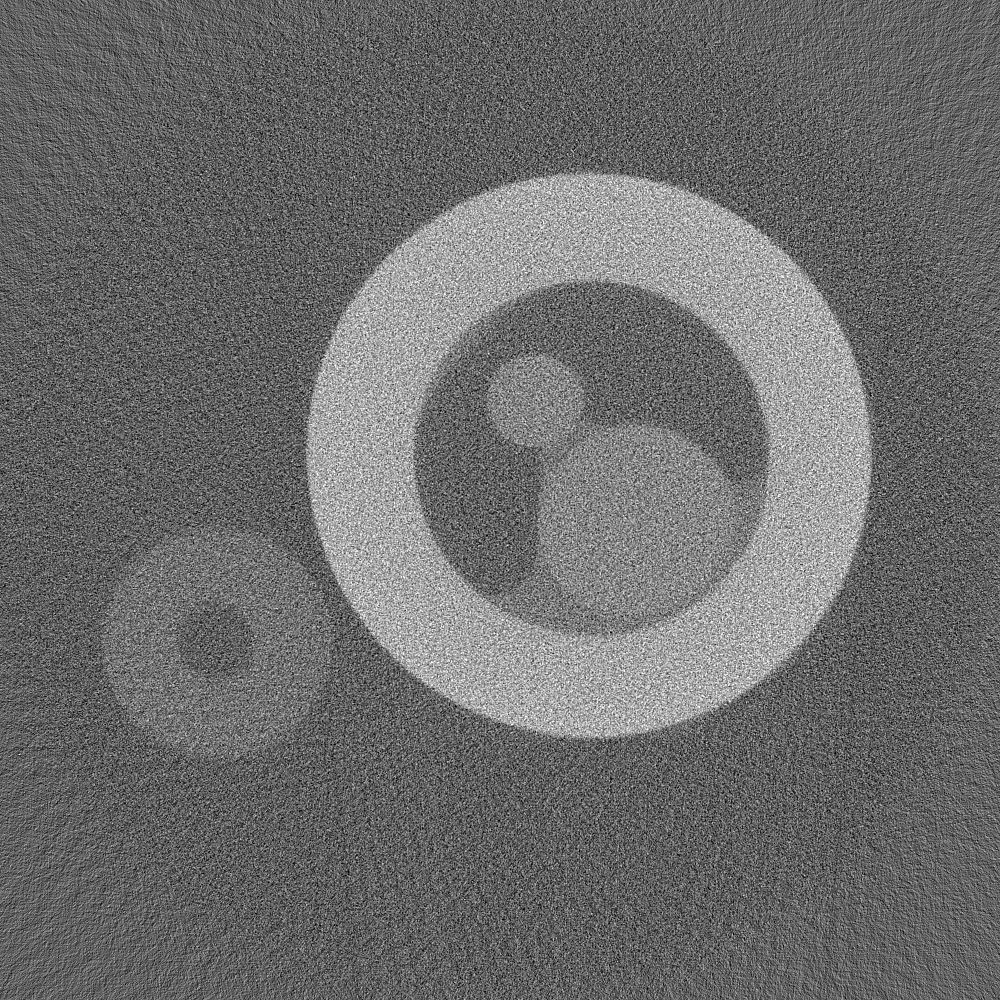
\includegraphics[width=\linewidth]{figures/kimrobertFDK.png}
      \caption{\acrlong{ihlq} \acrshort{fdk}.}
    \end{subfigure}
  
    \medskip
  
    \begin{subfigure}[t]{.45\textwidth}
      \centering
      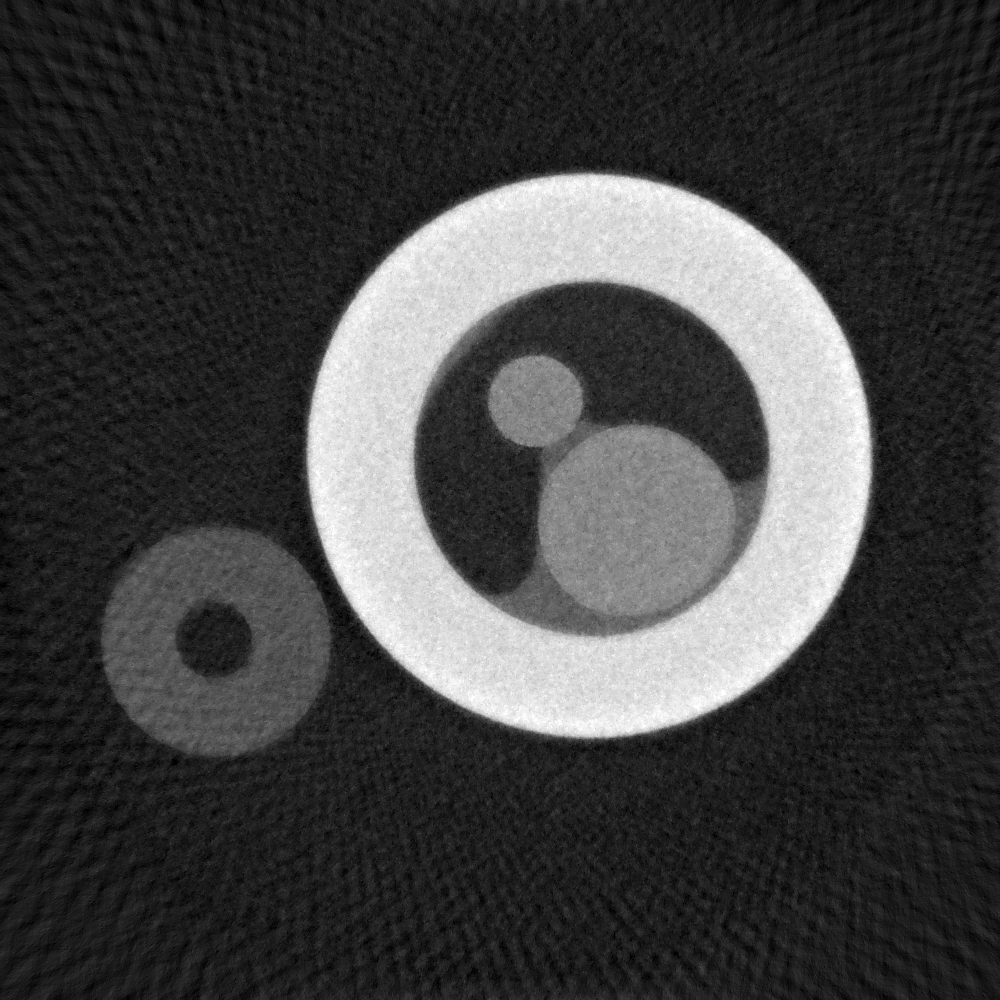
\includegraphics[width=\linewidth]{figures/kimrobertPICCS.png}
      \caption{\acrlong{ihlq} \acrshort{piccs}. }
    \end{subfigure}
    \hfill
    \begin{subfigure}[t]{.45\textwidth}
      \centering
      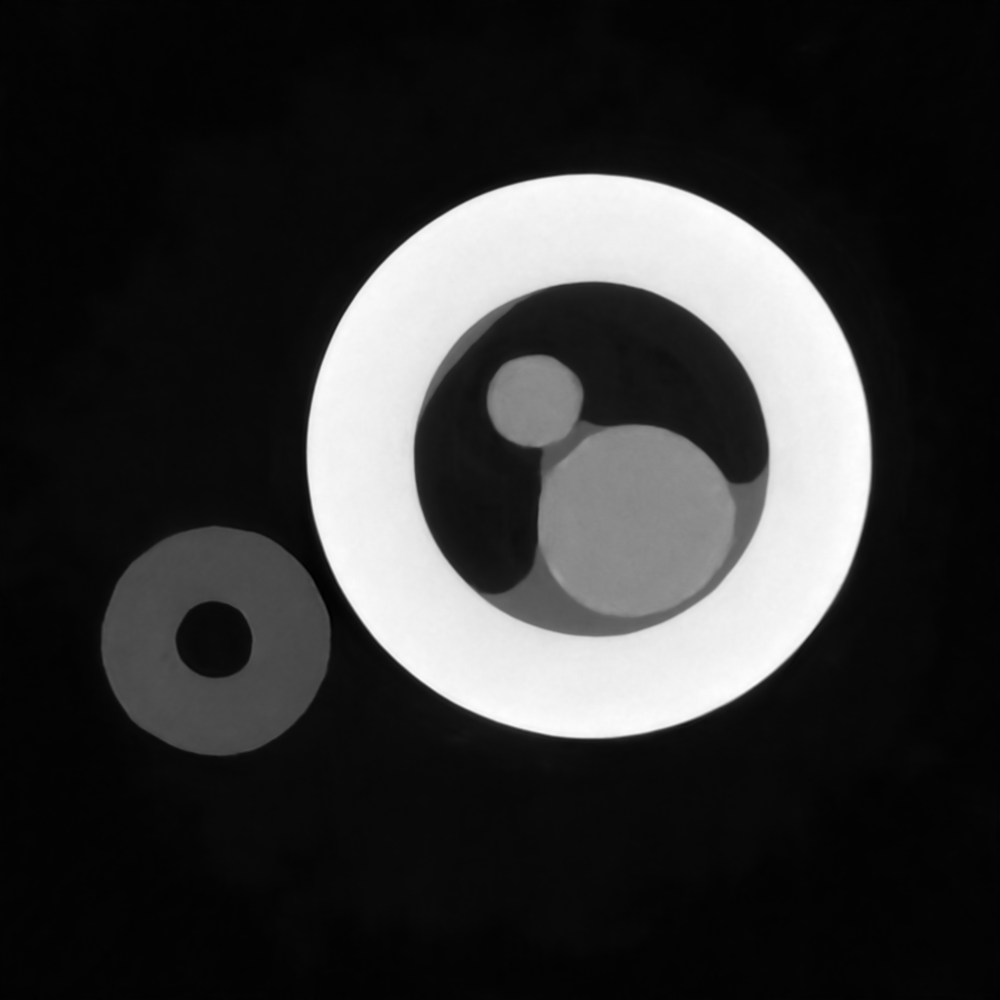
\includegraphics[width=\linewidth]{figures/kimrobertdepth1dn.png}
      \caption{\acrlong{dn} \acrlong{ihlq} \acrshort{fdk}. }
    \end{subfigure}
    \caption[Comparison of different reconstructions of IHHQ and IHLQ]{Comparison of different reconstructions of the \acrshort{ihhq} and the \acrshort{ihlq} dataset. }
    \label{fig:kimrobertcomparison}
\end{figure}
\todo[]{Remove \cref{fig:kimrobertcomparison}? May not be needed, as this is basically showed in other figures. }

\begin{figure}[htbp]
  \centering
  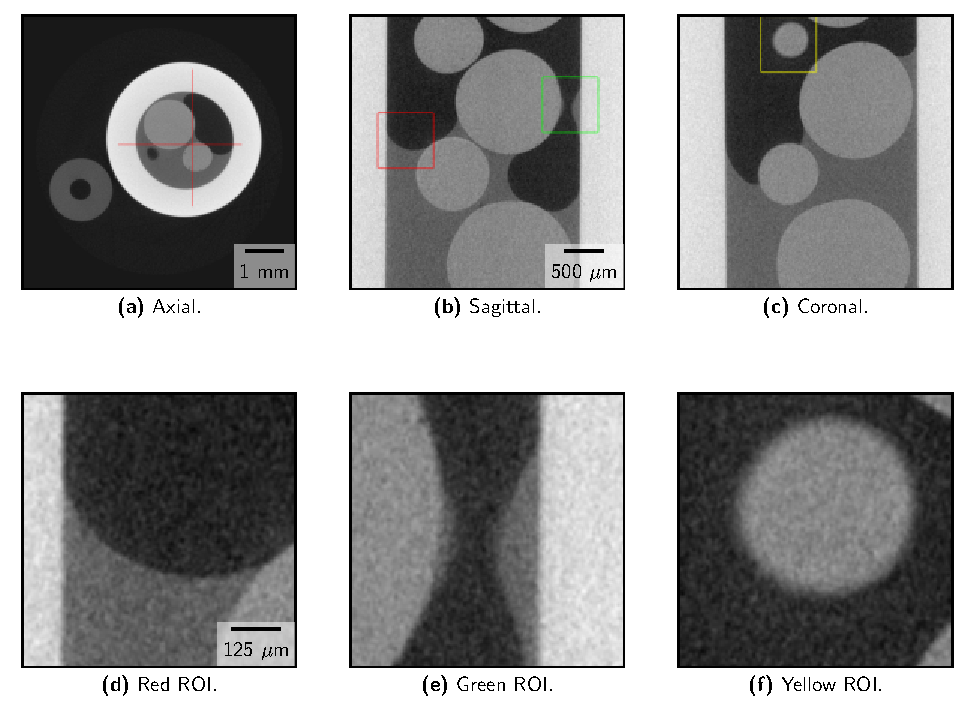
\includegraphics[width=.9\textwidth]{figures/kimroberthq-x475y620s250.pdf}
  \caption[View of IHHQ]{View of the \acrshort{ihhq} \acrshort{fdk} reconstruction. The red horizontal line in \textbf{(a)} corresponds to the sagittal view in \textbf{(b)}, and the red vertical line corresponds to the coronal view in \textbf{(c)}. Three \acrshort{roi}s have been marked in \textbf{(b)} and \textbf{(c)}, and can be seen in \textbf{(d)}-\textbf{(f)}. The scale bar for \textbf{(b)} applies to \textbf{(c)}, and the scale bar for \textbf{(d)} applies to \textbf{(e)} and \textbf{(f)}. }
  \label{fig:sideplothq}
\end{figure}

\begin{figure}[htbp]
  \centering
  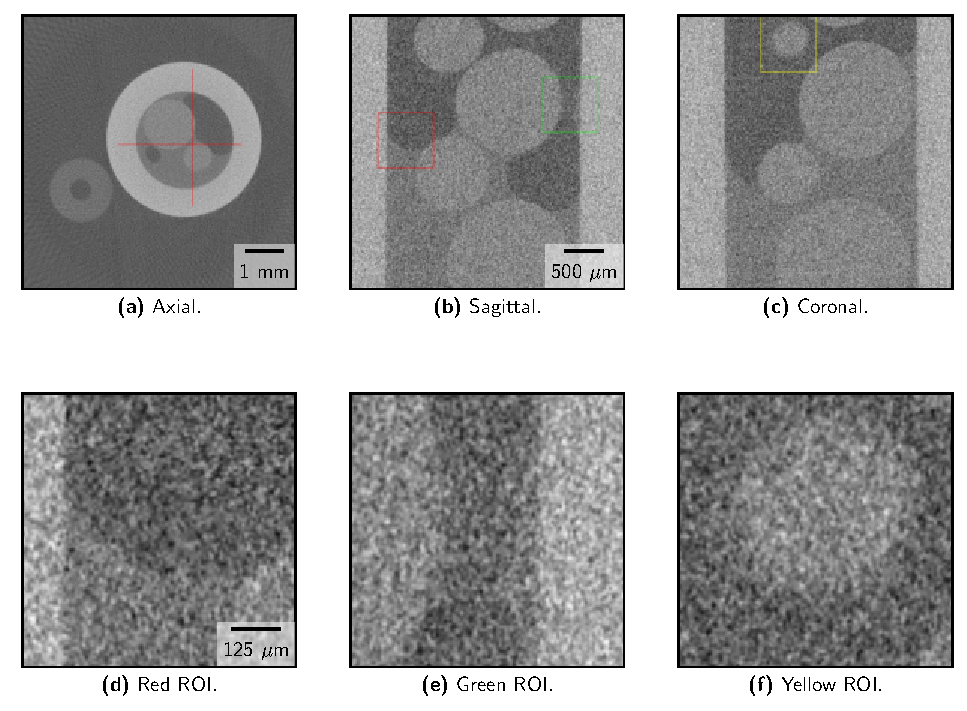
\includegraphics[width=.9\textwidth]{figures/kimrobertfdk-x475y620s250.pdf}
  \caption[View of IHLQ FDK]{View of the \acrshort{ihlq} \acrshort{fdk} reconstruction. Figure elements are as in \cref{fig:sideplothq}.} 
  \label{fig:sideplotfdk}
\end{figure}

\begin{figure}[htbp]
  \centering
  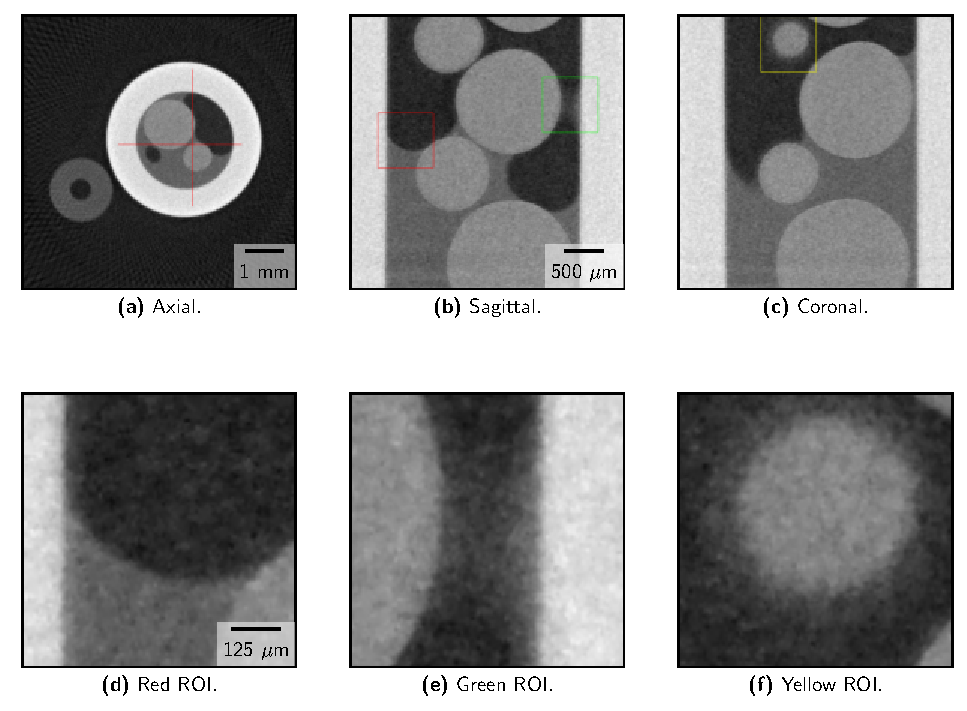
\includegraphics[width=.9\textwidth]{figures/kimrobertpiccs-x475y620s250.pdf}
  \caption[View of IHLQ PICCS]{View of the \acrshort{ihlq} \acrshort{piccs} reconstruction. Figure elements are as in \cref{fig:sideplothq}. }
  \label{fig:sideplotpiccs}
\end{figure}

\begin{figure}[htbp]
  \centering
  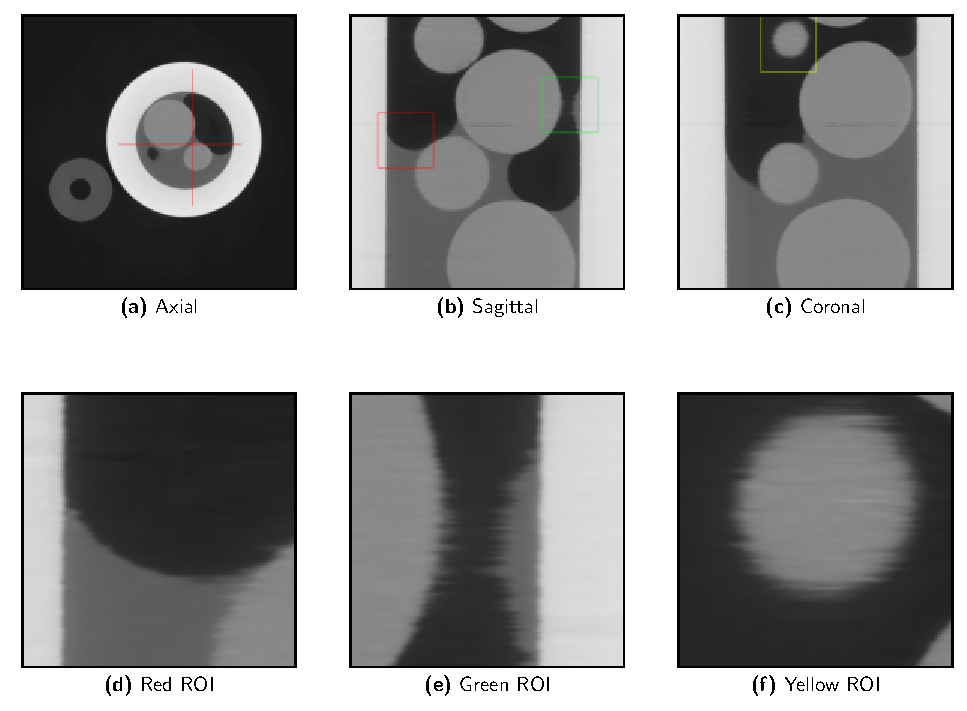
\includegraphics[width=.9\textwidth]{figures/kimrobertdepth1-x475y620s250.pdf}
  \caption[View of IHLQ FDK denoised with a depth of 1]{View of the denoised \acrshort{ihlq} \acrshort{fdk} reconstruction with a denoising depth of 1. Figure elements are as in \cref{fig:sideplothq}. }
  \label{fig:sideplotdepth1}
\end{figure}

\begin{figure}[htbp]
  \centering
  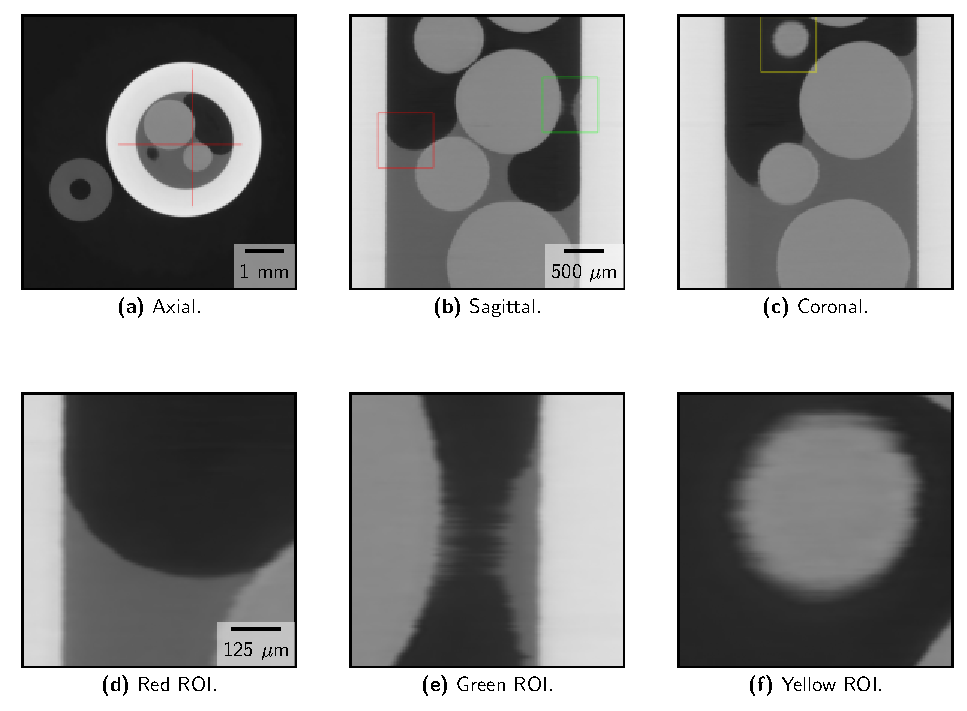
\includegraphics[width=.9\textwidth]{figures/kimrobertdepth3-x475y620s250.pdf}
  \caption[View of IHLQ FDK denoised with a depth of 3]{View of the denoised \acrshort{ihlq} \acrshort{fdk} reconstruction with a denoising depth of 3. Figure elements are as in \cref{fig:sideplothq}. }
  \label{fig:sideplotdepth3}
\end{figure}

\begin{figure}[htbp]
  \centering
  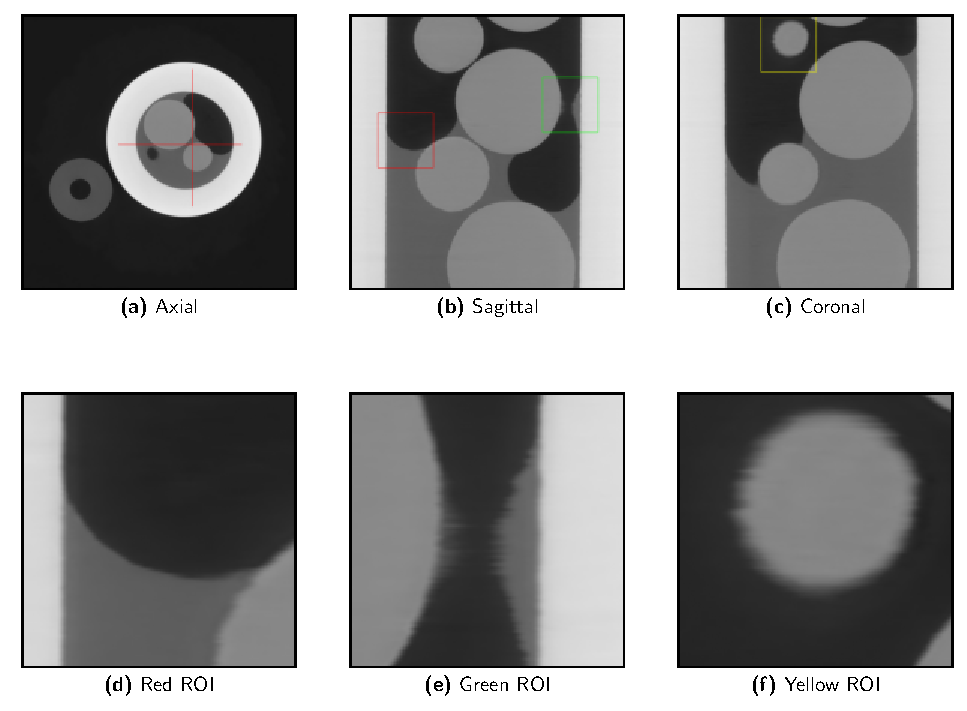
\includegraphics[width=.9\textwidth]{figures/kimrobertdepth5-x475y620s250.pdf}
  \caption[View of IHLQ FDK denoised with a depth of 5]{View of the denoised \acrshort{ihlq} \acrshort{fdk} reconstruction with a denoising depth of 5. Figure elements are as in \cref{fig:sideplothq}. }
  \label{fig:sideplotdepth5}
\end{figure}

\begin{figure}[htbp]
  \centering
  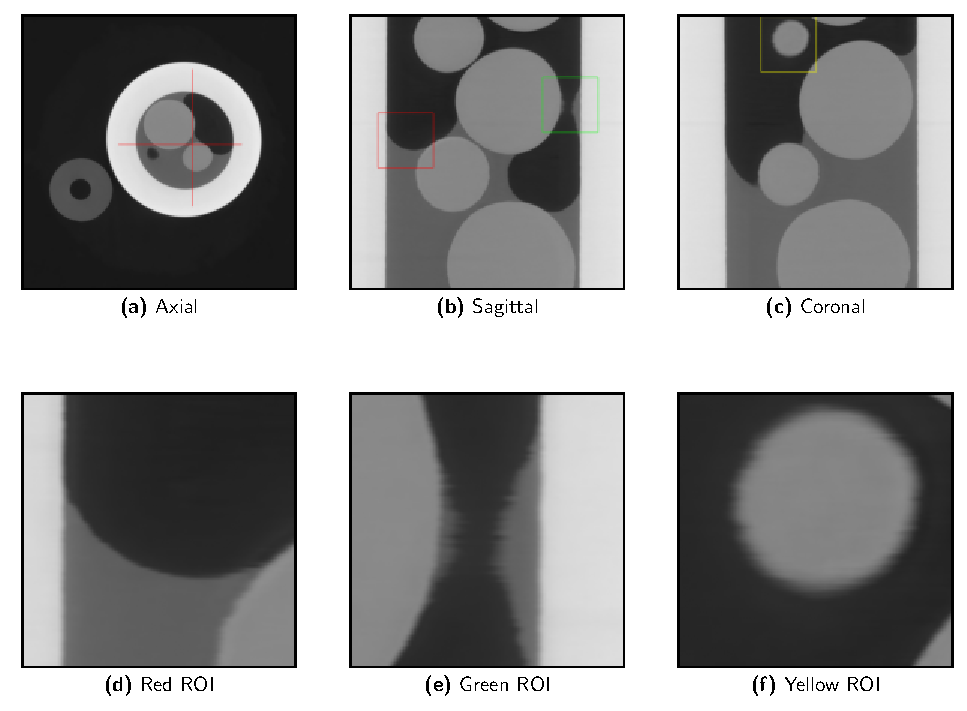
\includegraphics[width=.85\textwidth]{figures/kimrobertdepth7-x475y620s250.pdf}
  \caption[View of IHLQ FDK denoised with a depth of 7]{View of the denoised \acrshort{ihlq} \acrshort{fdk} reconstruction with a denoising depth of 7. Figure elements are as in \cref{fig:sideplothq}. }
  \label{fig:sideplotdepth7}
\end{figure}

\begin{figure}[htbp]
  \centering
  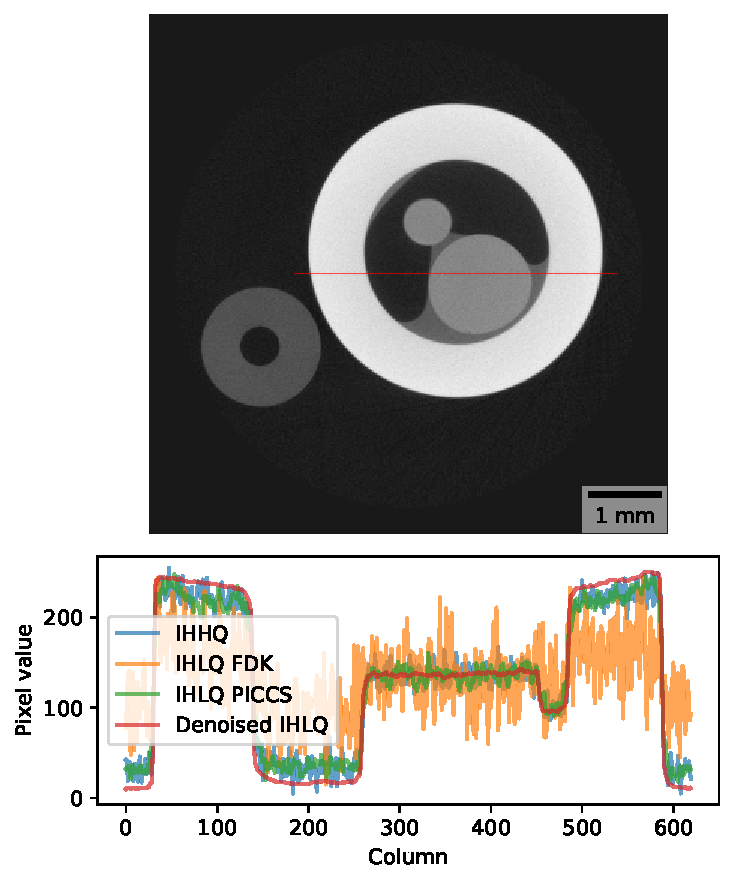
\includegraphics[width=.85\textwidth]{figures/kimrobertline.pdf}
  \caption[Line plot of IHHQ and IHLQ, noisy and denoised]{The plot shows pixel values for 620 pixels on a horizontal line, as shown by the red line on the \acrshort{hq} image above, on the \acrshort{ihhq} and \acrshort{ihlq} dataset, both noisy and denoised. The denoised values are from denoising the \acrshort{ihlq} \acrshort{fdk} reconstruction with TomoGAN using a loss function containing \acrshort{mse}, log-cosh, VGG, and adversarial loss components, a depth of 1, and the network was trained for $100 000$ iterations. }
  \label{fig:kimrobertline}
\end{figure}

\begin{figure}[htbp]
  \centering
  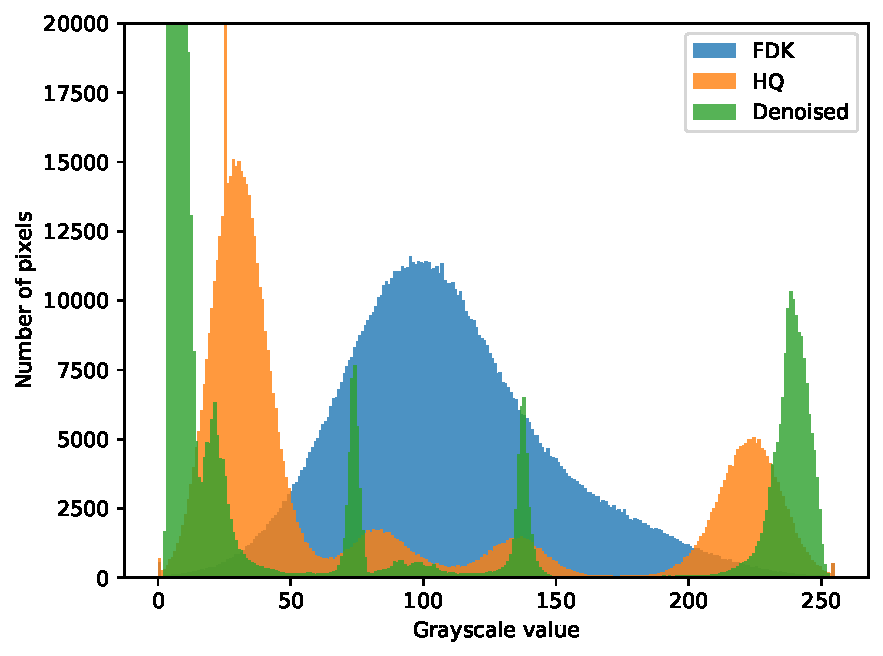
\includegraphics[width=.85\textwidth]{figures/kimroberthist.pdf}
  \caption[Histograms of IHHQ and IHLQ, noisy and denoised]{Histograms of the \acrshort{ihhq} and \acrshort{ihlq} \acrshort{fdk} dataset, both noisy and denoised. The denoising was done with TomoGAN using a loss function containing \acrshort{mse}, log-cosh, VGG, and adversarial loss components, a depth of 1, and the network was trained for $100 000$ iterations. Note that the ordinate has been cropped to a max value of $20000$. }
  \label{fig:kimroberthist}
\end{figure}

\section{Attempted Shale Denoising}
\todo[inline]{Shows limitations of method: requires a high-quality similar dataset (i.e. some ground truth) to work properly. Any given trained network doesn't work for all other dataset. }
\cref{fig:shale}

\begin{figure}
  \begin{subfigure}[t]{\textwidth}
    \centering
    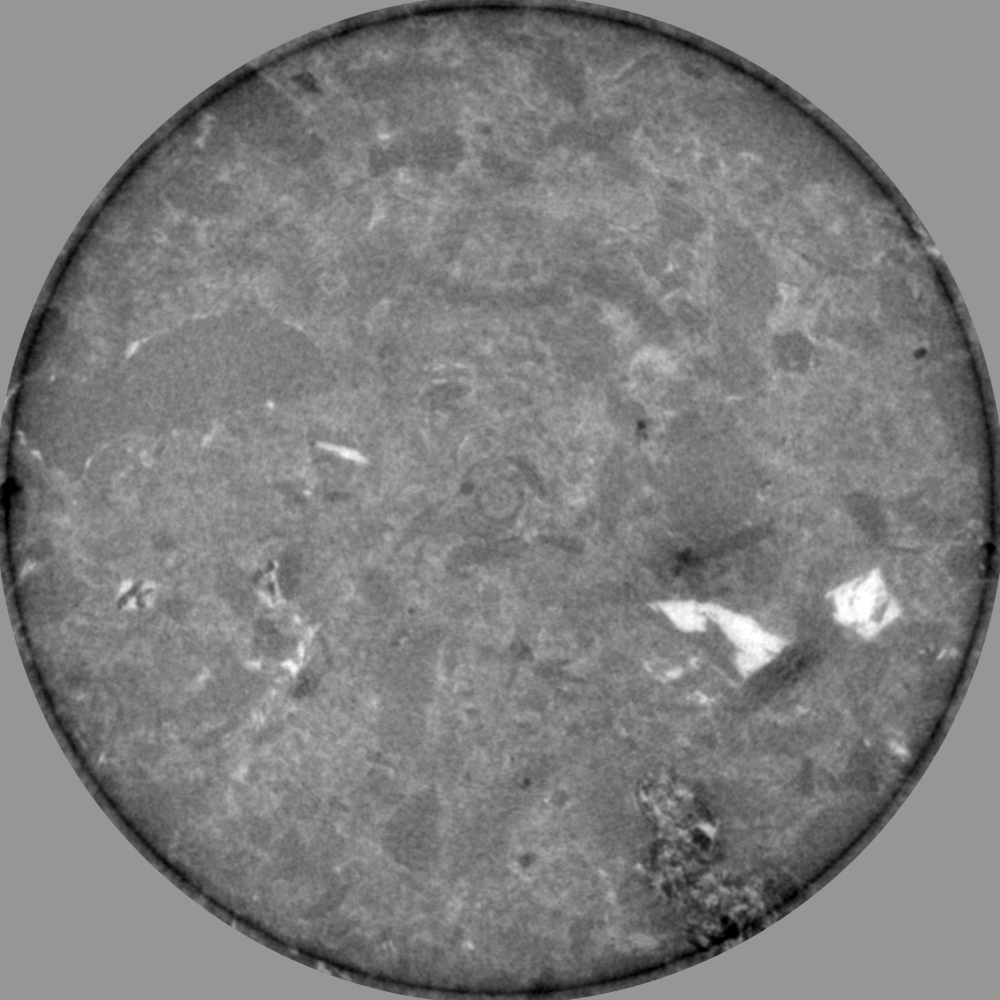
\includegraphics[width=.45\textwidth]{figures/shale/shale_ns/0.png}
    \caption{Original image. }
  \end{subfigure}

  \medskip

  \begin{subfigure}[t]{.45\textwidth}
    \centering
    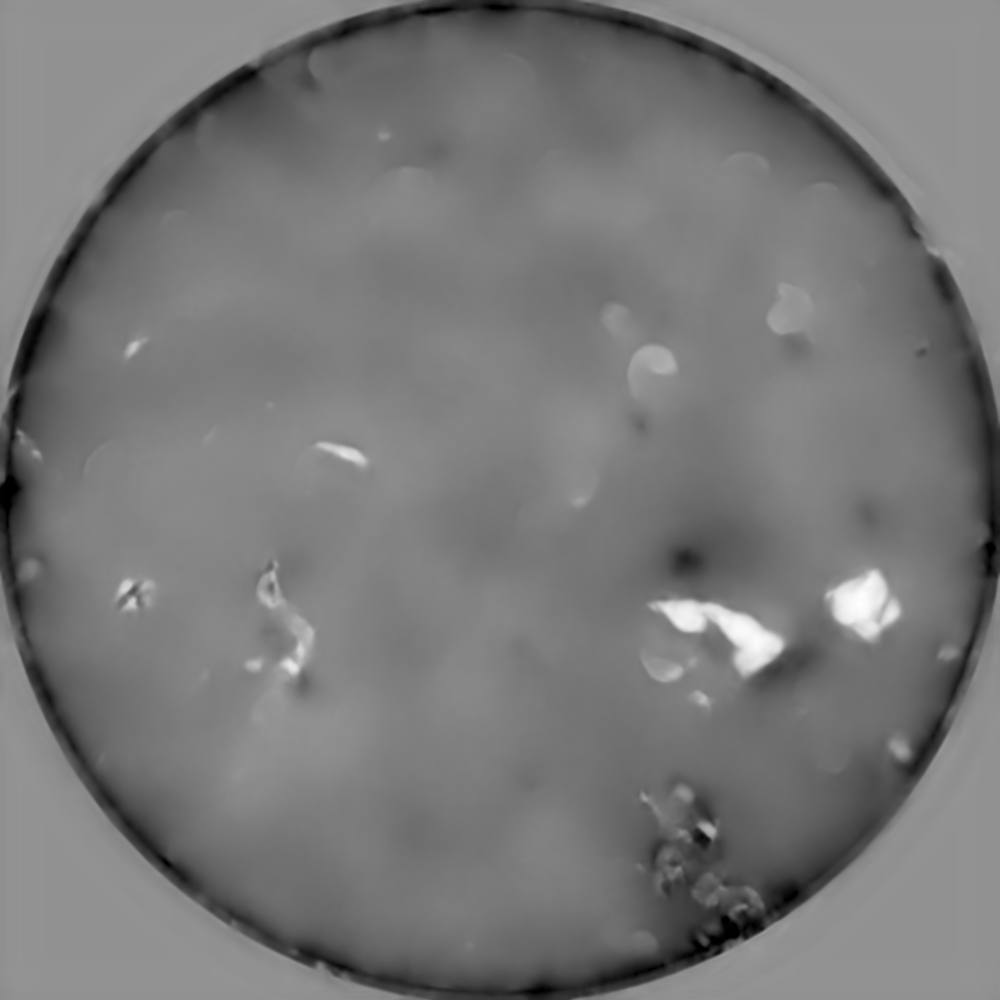
\includegraphics[width=\linewidth]{figures/shale/shale_dn_tomo00058/0.png}
    \caption{tomo\_00058. }
  \end{subfigure}
  \hfill
  \begin{subfigure}[t]{.45\textwidth}
    \centering
    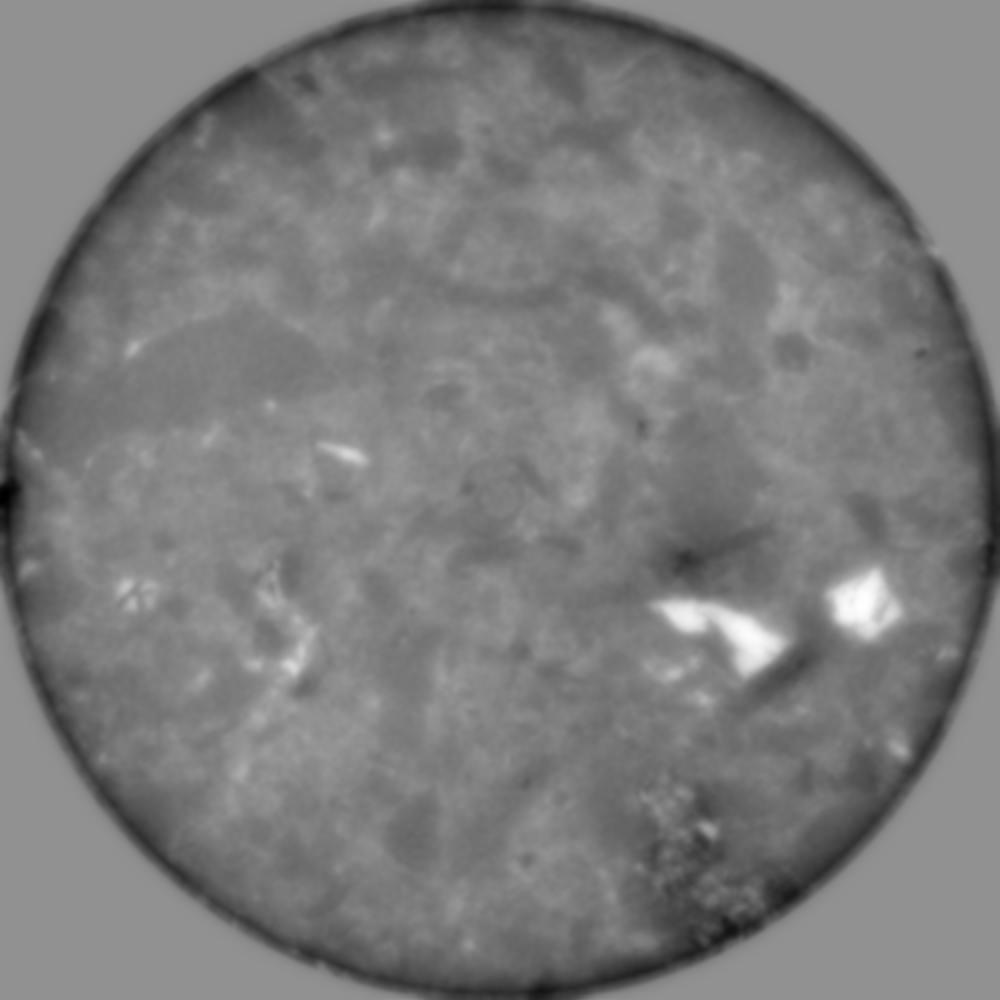
\includegraphics[width=\linewidth]{figures/shale/shale_dn_tomo00001/0.png}
    \caption{tomo\_00001. }
  \end{subfigure}

  \medskip

  \begin{subfigure}[t]{.45\textwidth}
    \centering
    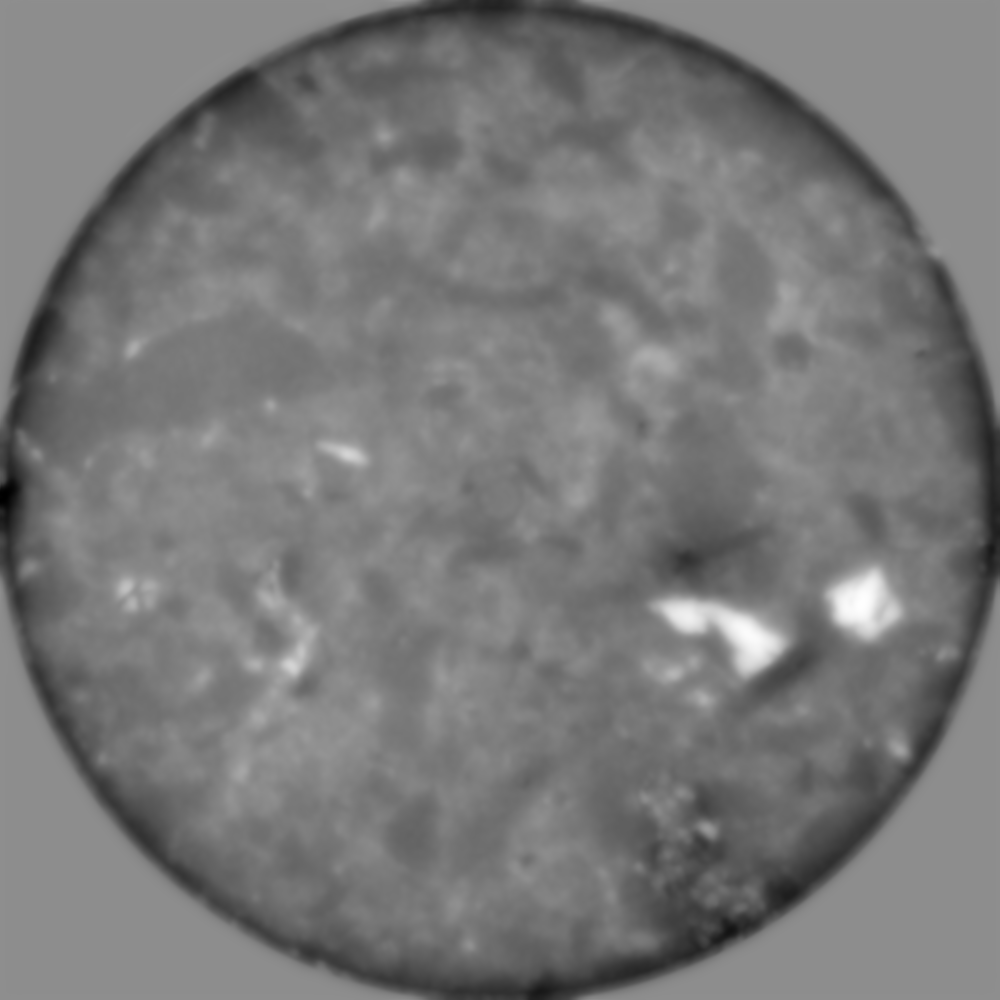
\includegraphics[width=\linewidth]{figures/shale/shale_dn_tomo00002/0.png}
    \caption{tomo\_00002. }
  \end{subfigure}
  \hfill
  \begin{subfigure}[t]{.45\textwidth}
    \centering
    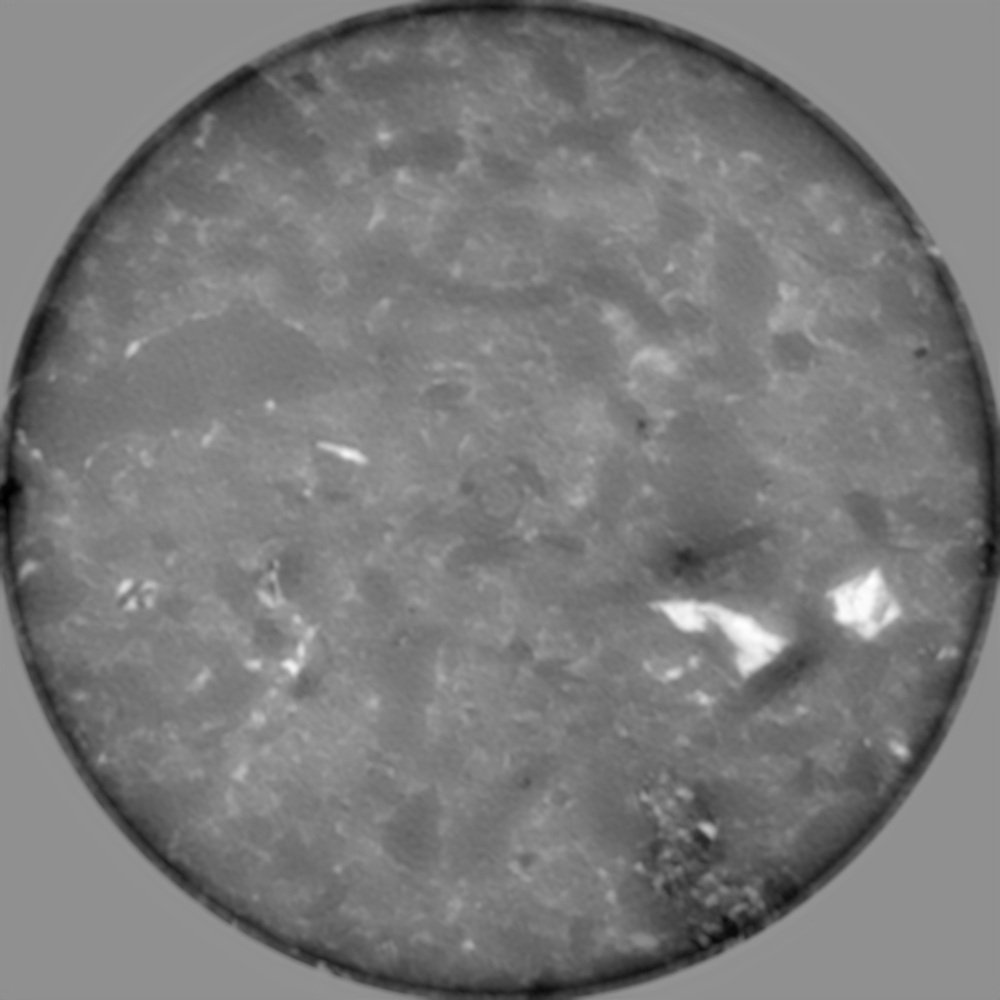
\includegraphics[width=\linewidth]{figures/shale/shale_dn_tomo00002min7/0.png}
    \caption{tomo\_00002min7. }
  \end{subfigure}
  \caption[Attempted shale denoising]{Attempted shale denoising. }
  \label{fig:shale}
\end{figure}




%Plot types: 
%\begin{itemize}
%    \item \acrshort{ssim} and \acrshort{mse} changes during training.
%    \item Loss function evolution.
%    \item Line plot of gt, ns, and different loss functions?
%    \item Histograms of gt, ns, denoised
%    \item Zoomed in region of interest.
%    \item Axial, sagittal, and coronal plots of (at least Kim Robert's dataset) different depth parameters.
%    \item Compare denoising of different subsamplings (8, 16, 32, 48)
%    \item Activation plot of network layers.
%\end{itemize}